\documentclass[14pt,a4paper]{extarticle}

\usepackage{fontspec}
\setmainfont{Times New Roman}
\setsansfont{Arial}
\setmonofont{Courier New}
\newfontfamily\cyrillicfonttt{Times New Roman}

\usepackage{polyglossia}
\setmainlanguage{russian}
\setotherlanguage{english}

\usepackage{geometry}
\geometry{left=30mm,right=15mm,top=20mm,bottom=20mm}

\usepackage{setspace}
\onehalfspacing

\usepackage{indentfirst}
\setlength{\parindent}{1.25cm}
\setlength{\parskip}{0pt}
\setlength{\emergencystretch}{2em}

\usepackage{graphicx}
\graphicspath{{figures/}}
\usepackage{float}
\usepackage{caption}
\DeclareCaptionLabelSeparator{emdash}{~---~}
\captionsetup{labelsep=emdash,justification=centering,singlelinecheck=false}
\captionsetup[table]{position=top}

\usepackage{array}
\usepackage{longtable}
\usepackage{tabularx}
\usepackage{booktabs}
\usepackage{multirow}
\usepackage{enumitem}
\usepackage{amsmath}
\usepackage{amssymb}
\usepackage{chngcntr}
\usepackage{titlesec}
\usepackage{fancyhdr}
\usepackage{hyperref}
\usepackage{verbatim}

\hypersetup{
    colorlinks=false,
    pdfborder={0 0 0}
}

\renewcommand{\textbf}[1]{#1}

\renewcommand{\thesection}{\arabic{section}}
\renewcommand{\thesubsection}{\thesection.\arabic{subsection}}
\renewcommand{\contentsname}{СОДЕРЖАНИЕ}

\titleformat{\section}
  {\normalfont\centering}
  {\thesection}
  {1em}
  {}

\titleformat{\subsection}
  {\normalfont}
  {\thesubsection}
  {1em}
  {}

\titlespacing*{\section}{0pt}{18pt}{12pt}
\titlespacing*{\subsection}{\parindent}{12pt}{6pt}

\pagestyle{fancy}
\fancyhf{}
\fancyfoot[C]{\thepage}
\renewcommand{\headrulewidth}{0pt}
\renewcommand{\footrulewidth}{0pt}

\begin{document}

\pagestyle{empty}
\newcommand{\maiheader}{
\begin{center}
\textbf{МИНИСТЕРСТВО НАУКИ И ВЫСШЕГО ОБРАЗОВАНИЯ}\\
\textbf{РОССИЙСКОЙ ФЕДЕРАЦИИ}\\[0.4em]
\textbf{ФЕДЕРАЛЬНОЕ ГОСУДАРСТВЕННОЕ БЮДЖЕТНОЕ ОБРАЗОВАТЕЛЬНОЕ}\\
\textbf{УЧРЕЖДЕНИЕ ВЫСШЕГО ОБРАЗОВАНИЯ}\\
\textbf{«МОСКОВСКИЙ АВИАЦИОННЫЙ ИНСТИТУТ}\\
\textbf{(национальный исследовательский университет)»}
\end{center}
}

\newcommand{\fieldline}[2]{\underline{\makebox[#1][l]{#2}}}

\thispagestyle{empty}
\small
\maiheader

\vspace{1.0em}
\noindent\textbf{Институт (Филиал) №8 «Компьютерные науки и прикладная математика»}\\
\textbf{Кафедра 806}\\
\textbf{Группа М8О-403Б-22}\\
\textbf{Направление подготовки 01.03.02 Прикладная математика и информатика}\\[0.3em]
\textbf{Профиль Информатика}\\[0.3em]
\textbf{Квалификация бакалавр}\\
\rule{2.5cm}{0.4pt}

\vspace{1.4em}
\begin{flushright}
\begin{tabular}{@{}lll@{}}
\textbf{УТВЕРЖДАЮ} & & \\
Заведующий кафедрой №806 & \fieldline{2.4cm}{} & С.\,С. Крылов \\
& {\scriptsize (№ каф.) \hspace{2.0cm} (подпись) \hspace{1.0cm} (инициалы, фамилия)} & \\
\fieldline{0.8cm}{} \hspace{0.3em} \fieldline{2.0cm}{} 2026 г. & &
\end{tabular}
\end{flushright}

\begin{center}
\textbf{ЗАДАНИЕ}\\
\textbf{на выпускную квалификационную работу}\\
\textbf{бакалавра}
\end{center}

\vspace{0.6em}
\noindent
\begin{tabularx}{\textwidth}{@{}lX@{}}
\textbf{Обучающийся} & \fieldline{10.5cm}{Мудров Павел Федорович} \\
& {\scriptsize (фамилия, имя, отчество полностью)} \\
\textbf{Руководитель} & \fieldline{10.5cm}{Ляпина Светлана Юрьевна} \\
& {\scriptsize (фамилия, имя, отчество полностью)} \\
\multicolumn{2}{@{}l@{}}{\fieldline{15.2cm}{профессор}} \\
\multicolumn{2}{@{}l@{}}{{\scriptsize ученая степень, ученое звание, должность и место работы}}
\end{tabularx}

\vspace{0.8em}
\noindent\textbf{1. Наименование темы}\hspace{0.8em}
«Применение методов обучения с подкреплением (Reinforcement Learning, RL) для прогнозирования и оптимизации биржевых котировок»

\vspace{0.8em}
\noindent\textbf{2. Срок сдачи обучающимся законченной работы}\hspace{0.8em}\fieldline{2.3cm}{15.05.2026}

\vspace{0.8em}
\noindent\textbf{3. Задание и исходные данные к работе}\\
Разработать единый экспериментальный стенд сравнения baseline-стратегий, статистических подходов, моделей машинного обучения и агентов обучения с подкреплением на биржевых котировках. Реализовать программный комплекс на Python с загрузкой данных, формированием признаков, обучением моделей, расчетом метрик и визуализацией результатов.

\vspace{0.3em}
\noindent\textbf{Перечень иллюстративно-графических материалов *при наличии:}

\vspace{0.3em}
\begin{center}
\begin{tabularx}{0.92\textwidth}{|c|X|c|}
\hline
№ п/п & Наименование & Количество листов \\
\hline
\rule{0pt}{1.4em} & & \\
\hline
\rule{0pt}{1.4em} & & \\
\hline
\rule{0pt}{1.4em} & & \\
\hline
\end{tabularx}
\end{center}

\newpage
\thispagestyle{empty}
\small

\noindent\textbf{4. Перечень подлежащих разработке разделов и этапы выполнения работы}

\vspace{0.4em}
\begin{center}
\setlength{\tabcolsep}{3pt}
\begin{tabularx}{0.92\textwidth}{|c|X|>{\centering\arraybackslash}p{2.3cm}|>{\centering\arraybackslash}p{2.6cm}|p{2.7cm}|}
\hline
№ п/п & Наименование раздела или этапа & Трудоемкость в \% от полной трудоемкости квалификационной работы & Срок выполнения & Примечание \\
\hline
1 & Анализ предметной области, аналогов и постановка исследовательской проблемы & 15 & 15.02.2026 & Выполнено на основе анализа литературы \\
\hline
2 & Проектирование экспериментального стенда и постановка задач ML и RL & 20 & 01.03.2026 & Согласовано с руководителем \\
\hline
3 & Реализация загрузки данных, генерации признаков, baseline-стратегий и ML-моделей & 25 & 20.03.2026 & Реализовано на языке Python \\
\hline
4 & Реализация RL-среды, обучение DQN и PPO, экспериментальное моделирование & 25 & 10.04.2026 & Проведено тестирование \\
\hline
5 & Подготовка выводов, оформление текста ВКР, рисунков и приложений & 15 & 15.05.2026 & Итоговое оформление работы \\
\hline
\end{tabularx}
\end{center}

\vspace{0.3em}
\noindent\textbf{5. Исходные материалы и пособия}
\begin{enumerate}[leftmargin=1.3cm,itemsep=0pt,topsep=0pt,label=\arabic*.]
\item Sutton R.\,S., Barto A.\,G. \textit{Reinforcement Learning: An Introduction}.
\item Hyndman R.\,J., Athanasopoulos G. \textit{Forecasting: Principles and Practice}.
\item Mnih V. et al. \textit{Human-level Control through Deep Reinforcement Learning}.
\item Schulman J. et al. \textit{Proximal Policy Optimization Algorithms}.
\item Документация \textit{stable-baselines3}, \textit{Gymnasium}, \textit{pandas}, \textit{scikit-learn}, \textit{yfinance}.
\end{enumerate}

\vspace{0.2em}
\noindent\textbf{6. Дата выдачи задания}\hspace{0.8em}\fieldline{2.3cm}{11.02.2026}

\vspace{0.6em}
\begin{tabularx}{\textwidth}{@{}X X@{}}
Руководитель \fieldline{4.3cm}{} & Задание принял к исполнению \fieldline{4.3cm}{} \\
{\scriptsize (подпись)} & {\scriptsize (подпись)}
\end{tabularx}

\newpage
\thispagestyle{empty}
\small
\maiheader

\vspace{1.0em}
\noindent\textbf{Институт (Филиал) №8 «Компьютерные науки и прикладная математика»}\\
\textbf{Кафедра 806}\\
\textbf{Группа М8О-403Б-22}\\
\textbf{Направление подготовки 01.03.02 Прикладная математика и информатика}\\[0.3em]
\textbf{Профиль Информатика}\\[0.3em]
\textbf{Квалификация бакалавр}

\vspace{1.8em}
\begin{center}
\textbf{ВЫПУСКНАЯ КВАЛИФИКАЦИОННАЯ РАБОТА}\\
\textbf{БАКАЛАВРА}
\end{center}

\vspace{0.8em}
\noindent
На тему: «Применение методов обучения с подкреплением (Reinforcement Learning, RL) для прогнозирования и оптимизации биржевых котировок»

\vspace{2.2em}
\noindent
Автор ВКРБ \fieldline{4.0cm}{} Мудров Павел Федорович\\
\hspace*{3.6cm}(\fieldline{1.5cm}{}) \hspace{3.0cm}{\scriptsize (фамилия, имя, отчество полностью)}\\[0.7em]
Руководитель \fieldline{3.2cm}{} Ляпина Светлана Юрьевна\\
\hspace*{3.7cm}(\fieldline{1.5cm}{}) \hspace{2.9cm}{\scriptsize (фамилия, имя, отчество полностью)}\\[0.7em]
Консультант \fieldline{3.1cm}{} \fieldline{6.2cm}{}\\
\hspace*{3.7cm}(\fieldline{1.5cm}{}) \hspace{2.9cm}{\scriptsize (фамилия, имя, отчество полностью)}\\[0.7em]
Консультант \fieldline{3.1cm}{} \fieldline{6.2cm}{}\\
\hspace*{3.7cm}(\fieldline{1.5cm}{}) \hspace{2.9cm}{\scriptsize (фамилия, имя, отчество полностью)}\\[0.7em]
Рецензент \fieldline{3.4cm}{} \fieldline{6.2cm}{}\\
\hspace*{3.7cm}(\fieldline{1.5cm}{}) \hspace{2.9cm}{\scriptsize (фамилия, имя, отчество полностью)}

\vspace{0.8em}
\noindent
\textbf{К защите допустить}\\
Заведующий кафедрой № 806 \hspace{0.8em} Крылов Сергей Сергеевич \hspace{0.8em} (\fieldline{1.6cm}{})\\
\hspace*{5.0cm}{\scriptsize (№ каф.) \hspace{3.2cm} (фамилия, имя, отчество полностью)}\\
\fieldline{0.8cm}{} \hspace{0.3em} \fieldline{2.3cm}{} 2026 г.

\vspace{1.0em}
\begin{center}
Москва 2026
\end{center}

\newpage
\thispagestyle{empty}
\normalsize
\begin{center}
\textbf{СПИСОК ИСПОЛНИТЕЛЕЙ}
\end{center}

\noindent
В выполнении выпускной квалификационной работы принимали участие:

\vspace{0.8em}
\noindent
Обучающийся --- Мудров Павел Федорович

\noindent
Руководитель --- Ляпина Светлана Юрьевна, профессор

\noindent
Консультант --- TODO: заполнить сведения при наличии

\noindent
Рецензент --- TODO: заполнить сведения при наличии

\newpage
\thispagestyle{empty}
\normalsize
\begin{center}
\textbf{РЕФЕРАТ}
\end{center}

\noindent
Выпускная квалификационная работа бакалавра состоит из 57 страниц, 28 использованных источников, 7 таблиц, 5 рисунков и одного приложения.

\vspace{0.5em}
\noindent
\textbf{ОБУЧЕНИЕ С ПОДКРЕПЛЕНИЕМ, БИРЖЕВЫЕ КОТИРОВКИ, АЛГОРИТМИЧЕСКАЯ ТОРГОВЛЯ, DQN, PPO, BASELINE-СТРАТЕГИИ, МАШИННОЕ ОБУЧЕНИЕ, ФИНАНСОВЫЕ МЕТРИКИ, EQUITY CURVE, MAX DRAWDOWN}

\vspace{0.5em}
\noindent
Работа посвящена исследованию применения методов обучения с подкреплением для прогнозирования и оптимизации торговых решений на биржевых котировках. В отличие от подходов, ориентированных исключительно на прогноз будущей цены, в работе рассматривается задача последовательного выбора действий \textit{buy}, \textit{sell} и \textit{hold} с учетом состояния рынка и динамики портфеля.

\noindent
В теоретической части рассмотрены особенности финансовых временных рядов, классические статистические методы, модели машинного обучения, нейросетевые подходы и современные RL-алгоритмы. Особое внимание уделено сравнению аналогов и формулированию проблемы, состоящей в том, что высокая точность прогноза не гарантирует практической прибыльности стратегии. На этой основе обоснована необходимость построения единого экспериментального стенда, в котором baseline-стратегии, ML-модели и RL-агенты оцениваются на одних и тех же данных и по единому набору метрик.

\noindent
В практической части описан программный проект на Python, включающий загрузку данных через \textit{yfinance}, генерацию признаков на основе OHLCV-рядов, реализацию стратегий \textit{Buy \& Hold} и \textit{Moving Average Crossover}, обучение моделей \textit{Logistic Regression}, \textit{Random Forest}, \textit{Gradient Boosting}, а также обучение агентов \textit{DQN} и \textit{PPO} в среде \textit{Gymnasium}. Для оценки результатов используются как ML-метрики, так и финансовые показатели: доходность, волатильность, коэффициент Шарпа, максимальная просадка и устойчивость стратегии.

\noindent
Результаты экспериментального моделирования показывают, что RL-подходы целесообразно рассматривать как инструмент оптимизации последовательных торговых решений, однако их качество существенно зависит от функции вознаграждения, набора признаков и рыночного режима. В условиях исследуемого стенда PPO-агент обеспечивает более устойчивый риск-скорректированный результат по сравнению с рядом альтернатив, тогда как стратегия \textit{Buy \& Hold} сохраняет преимущество по абсолютной доходности на выраженном восходящем рынке.


\clearpage
\pagestyle{empty}
\tableofcontents

\clearpage
\clearpage
\section*{ТЕРМИНЫ И ОПРЕДЕЛЕНИЯ}
\addtocontents{toc}{\protect\contentsline{section}{ТЕРМИНЫ И ОПРЕДЕЛЕНИЯ}{}{}}

В настоящей выпускной квалификационной работе применяют следующие термины с соответствующими определениями:

\textbf{Биржевая котировка} — опубликованное во времени значение цены финансового инструмента, сформированное в результате биржевых сделок и используемое для анализа рыночной динамики

\textbf{Финансовый временной ряд} — упорядоченная по времени последовательность наблюдений за рыночными переменными, такими как цена открытия, максимум, минимум, цена закрытия и объем торгов

\textbf{OHLCV-данные} — формат представления рыночной информации, включающий цену открытия (\textit{Open}), максимум (\textit{High}), минимум (\textit{Low}), цену закрытия (\textit{Close}) и объем торгов (\textit{Volume})

\textbf{Торговая стратегия} — формализованный набор правил, определяющий условия открытия, удержания и закрытия позиции на финансовом рынке

\textbf{Baseline-стратегия} — простая эталонная стратегия, используемая как нижняя граница качества при сравнении более сложных алгоритмов

\textbf{Признак} — числовая характеристика состояния рынка, используемая моделью для принятия решения или прогнозирования

\textbf{Целевая переменная} — величина, которую модель должна предсказать, например направление изменения цены или доходность следующего периода

\textbf{Обучение с подкреплением} — парадигма машинного обучения, при которой агент последовательно взаимодействует со средой, выбирает действия и получает награду за последствия этих действий

\textbf{Агент} — обучаемая система, принимающая решения в среде на основе наблюдаемого состояния

\textbf{Состояние среды} — совокупность признаков, описывающих доступную агенту информацию о рынке и текущем состоянии портфеля

\textbf{Функция вознаграждения} — правило количественной оценки результата действия агента, используемое для настройки его поведения

\textbf{Equity curve} — кривая стоимости портфеля во времени, отражающая изменение капитала при выполнении стратегии

\textbf{Просадка} — относительное снижение стоимости портфеля от локального максимума до последующего минимума

\clearpage
\section*{ПЕРЕЧЕНЬ СОКРАЩЕНИЙ И ОБОЗНАЧЕНИЙ}
\addtocontents{toc}{\protect\contentsline{section}{ПЕРЕЧЕНЬ СОКРАЩЕНИЙ И ОБОЗНАЧЕНИЙ}{}{}}

В настоящей выпускной квалификационной работе применяют следующие сокращения и обозначения:

ИИ — искусственный интеллект

МО — машинное обучение

RL — reinforcement learning, обучение с подкреплением

DL — deep learning, глубокое обучение

OHLCV — open, high, low, close, volume

SMA — simple moving average, простое скользящее среднее

RSI — relative strength index

MACD — moving average convergence divergence

ARIMA — autoregressive integrated moving average

SARIMA — seasonal autoregressive integrated moving average

LSTM — long short-term memory

GRU — gated recurrent unit

DQN — deep Q-network

PPO — proximal policy optimization

A2C — advantage actor-critic

ROC-AUC — area under the receiver operating characteristic curve

MDP — Markov decision process

API — application programming interface


\clearpage
\pagenumbering{arabic}
\setcounter{page}{1}
\pagestyle{fancy}
\clearpage
\section*{ВВЕДЕНИЕ}
\addcontentsline{toc}{section}{ВВЕДЕНИЕ}

Современные финансовые рынки характеризуются высокой скоростью обновления информации, существенной изменчивостью цен и постоянной конкуренцией между участниками, использующими различные аналитические и вычислительные методы. В этой среде задача прогнозирования биржевых котировок остается одной из ключевых как для прикладной финансовой аналитики, так и для области искусственного интеллекта. Однако накопленный опыт показывает, что сама по себе задача прогноза цены не исчерпывает практическую постановку проблемы. Даже при наличии модели, демонстрирующей приемлемое качество по статистическим критериям, ее полезность для принятия торговых решений может оказаться ограниченной. Модель может корректно предсказывать направление части движений, но при этом формировать чрезмерно частые сигналы, создавать высокую просадку или не учитывать транзакционные издержки [3, 6, 7].

Актуальность темы определяется сразу несколькими обстоятельствами. Во-первых, финансовые временные ряды являются типичным примером сложных нестационарных данных, для которых недостаточно только классических статистических методов. Во-вторых, широкое распространение получили модели машинного обучения и глубокого обучения, ориентированные на выделение сложных зависимостей в данных. В-третьих, в последние годы заметно вырос интерес к обучению с подкреплением как к подходу, который позволяет не просто прогнозировать цену, а обучать агента непосредственному выбору действий на рынке. Для задач алгоритмической торговли это особенно важно, поскольку конечная цель практической системы состоит не в минимизации ошибки прогноза как таковой, а в повышении эффективности последовательных торговых решений с учетом риска, просадки, комиссий и устойчивости поведения на различных рыночных режимах [3, 7, 11, 12, 21].

Дополнительную значимость теме придает замечание, сделанное научным руководителем: при обосновании актуальности необходимо не только описать применимость RL-подходов, но и провести сравнение существующих аналогов, а также четко показать проблему, которую решает работа. Действительно, без такого сравнения исследование рискует превратиться в изолированное описание одного алгоритма. Поэтому в настоящей работе обучение с подкреплением рассматривается не как самоцель, а как один из классов методов, сопоставляемый с традиционными baseline-стратегиями, статистическими моделями и классическими алгоритмами машинного обучения в рамках единого экспериментального стенда.

Проблема исследования состоит в следующем. Большинство подходов к анализу биржевых данных оцениваются либо по ошибке прогноза, либо по отдельным финансовым показателям, но не всегда в рамках единой методологии. На практике это приводит к нескольким методологическим трудностям. Во-первых, сравнение моделей оказывается некорректным, если они обучаются и тестируются на разных интервалах или по разным правилам формирования сигналов. Во-вторых, высокая классификационная точность не эквивалентна высокой доходности стратегии, поскольку итоговый результат зависит от частоты сделок, величины прибыли на одну сделку, транзакционных издержек и характера рыночного режима. В-третьих, многие работы рассматривают RL-агентов обособленно, без сопоставления с простыми и интерпретируемыми альтернативами, такими как Buy \& Hold или стратегия на пересечении скользящих средних [6, 7, 27, 28].

Таким образом, возникает необходимость в разработке программного решения, которое позволяет на едином наборе биржевых данных формировать признаки, обучать модели, запускать алгоритмы принятия торговых решений, выполнять backtesting и рассчитывать показатели качества по единым правилам. Именно создание и экспериментальная проверка такого решения составляют центральное содержание настоящей выпускной квалификационной работы.

Целью работы является разработка, программная реализация и экспериментальная проверка программного решения для прогнозирования и оптимизации торговых решений на основе биржевых котировок с использованием baseline-стратегий, моделей машинного обучения и методов обучения с подкреплением.

Для достижения поставленной цели в работе решаются следующие задачи:
\begin{enumerate}[leftmargin=1.25cm,label=\arabic*)]
\item проанализировать особенности биржевых котировок как финансовых временных рядов и определить требования к разрабатываемому программному решению;
\item выполнить обзор существующих подходов и аналогов, необходимых для выбора состава реализуемых модулей и методов сравнения;
\item спроектировать архитектуру программного решения, включающего загрузку данных, формирование признаков, модуль принятия решений и подсистему оценки результатов;
\item реализовать модуль подготовки OHLCV-данных, модуль генерации признаков, baseline-стратегии, классические ML-модели и RL-среду для обучения агентов DQN и PPO;
\item формализовать задачу обучения с подкреплением, включая описание состояния среды, пространства действий, функции вознаграждения и ограничений торговой логики;
\item реализовать процедуры обучения, тестирования и backtesting, обеспечивающие воспроизводимый запуск вычислительного эксперимента;
\item провести экспериментальную проверку разработанного программного решения и сравнить реализованные подходы по классификационным и финансовым метрикам;
\item выполнить анализ полученных результатов, определить ограничения решения и наметить направления его дальнейшего развития.
\end{enumerate}

Объектом исследования являются методы анализа и принятия решений на основе биржевых котировок.

Предметом исследования выступают алгоритмы прогнозирования и оптимизации торговых стратегий на финансовых временных рядах, в том числе baseline-подходы, модели машинного обучения и методы обучения с подкреплением.

В работе применяются методы статистического анализа временных рядов, методы машинного обучения, методы обучения с подкреплением, методы финансовой оценки торговых стратегий, а также методы программной инженерии для построения воспроизводимого вычислительного контура. Практическая реализация выполнена на языке Python с использованием библиотек \textit{pandas}, \textit{NumPy}, \textit{scikit-learn}, \textit{yfinance}, \textit{Gymnasium}, \textit{stable-baselines3} и \textit{matplotlib} [15, 16, 17, 19, 20, 24].

Практическая значимость работы заключается в создании работоспособного программного решения, пригодного для воспроизводимого запуска экспериментов по алгоритмической торговле на исторических котировках. Разработанный pipeline позволяет автоматически загружать данные, формировать признаки, обучать реализованные модели, запускать стратегии на тестовом интервале, рассчитывать финансовые показатели и сохранять результаты в виде отчетных артефактов. Такой подход представляет интерес как для учебных целей, так и для дальнейшего наращивания функциональности за счет новых признаков, алгоритмов и сценариев оценки.

Научная новизна работы в рамках учебного исследования состоит в том, что RL-подход рассматривается не изолированно, а как часть разработанного программного контура, в котором прогнозирующие модели и торговые стратегии сравниваются по единым правилам входных данных, тестирования и расчета метрик. Это позволяет сместить акцент с абстрактного качества прогноза на более прикладной вопрос: может ли реализованный RL-агент улучшить не только точность сигнала, но и риск-скорректированную результативность торговой системы.

Структурно работа включает введение, четыре главы, заключение, список использованных источников и приложение. В первой главе рассматриваются предметная область, существующие подходы и аналоги, а также формулируется проблема исследования. Во второй главе описываются проектирование метода, подготовка данных, признаки, постановка RL-задачи и система метрик. Третья глава посвящена реализации программного решения и экспериментального стенда. В четвертой главе представлены результаты экспериментального моделирования, их сопоставление и интерпретация. В заключении сформулированы основные результаты, ограничения и направления дальнейшего развития работы.

\clearpage
\section{АНАЛИЗ ПРЕДМЕТНОЙ ОБЛАСТИ И СУЩЕСТВУЮЩИХ АНАЛОГОВ}

\subsection{Особенности биржевых котировок как временных рядов}

Биржевые котировки относятся к классу финансовых временных рядов, для которых характерно сочетание трендовых участков, шумовой компоненты, изменения волатильности и зависимости от внешних новостных и макроэкономических факторов. В отличие от многих инженерных временных рядов, в рыночных данных редко выполняется предположение о строгой стационарности. Распределение доходностей может меняться во времени, амплитуда колебаний возрастает в периоды стрессов, а закономерности, найденные на одном интервале, часто деградируют на другом. Это явление в прикладных работах связывают с изменением рыночного режима и эффектом \textit{concept drift} [3, 25, 26].

С практической точки зрения биржевой ряд представляет собой не просто последовательность значений цены, а комплексную динамическую систему, где существенную роль играют доходности, скорость изменения цены, локальный тренд, объемы торгов и взаимодействие нескольких временных масштабов. Для целей построения торговых стратегий важны не только ожидаемый уровень цены, но и вероятность благоприятного движения в ближайшем будущем, вероятность ложного сигнала, длительность удержания позиции и ожидаемая величина просадки. Вследствие этого выбор модели должен учитывать как прогностическую силу признаков, так и последующее влияние предсказаний на торговый контур [3, 6].

Дополнительная сложность заключается в том, что на финансовых рынках высокая ошибка в несколько отдельных моментов способна перечеркнуть полезность большого числа корректных прогнозов. Например, стратегия может правильно предсказывать большую долю небольших движений, но потерять значительную часть капитала на редких сильных разворотах. Поэтому интерпретация качества модели через одну лишь среднюю ошибку или точность классификации является неполной. Для корректного исследования необходимо переходить от анализа ряда как статистического объекта к анализу результата как динамики стоимости портфеля [7, 27, 28].

\subsection{Классические методы прогнозирования финансовых временных рядов}

Классические методы прогнозирования финансовых временных рядов включают наивные стратегии, модели сглаживания, авторегрессионные модели и сезонные модификации, такие как ARIMA и SARIMA. Их достоинство состоит в хорошо разработанном математическом аппарате, интерпретируемости параметров и понятной процедуре оценки. Для многих экономических и производственных рядов такие модели остаются надежным инструментом. Однако в отношении биржевых котировок их применимость ограничивается тем, что динамика цен часто содержит выраженную нелинейность, структурные сдвиги и слабую устойчивость локальных закономерностей [2, 4].

Наивная модель \textit{random walk}, предполагающая, что лучшее предсказание следующего значения равно текущему, долгое время использовалась как базовая точка отсчета для оценки более сложных алгоритмов. В рамках торговли ей соответствует \textit{Buy \& Hold}, если актив находится в долгосрочном восходящем тренде, или пассивное отсутствие позиции, если цель исследования сводится к прогнозированию самого уровня цены. Скользящие средние, экспоненциальное сглаживание и ARIMA-подходы позволяют выделять локальные зависимости, но плохо переносят резкие изменения режима, характерные для финансовых рынков [4, 25, 26].

В контексте настоящей работы классические статистические модели важны по двум причинам. Во-первых, они задают нижнюю и среднюю планку для сравнения более современных методов. Во-вторых, они демонстрируют ограничение постановки, в которой цель исследования сводится исключительно к прогнозу следующего значения ряда. Даже хорошо подогнанная ARIMA-модель не определяет напрямую, когда открывать позицию, как долго ее удерживать и как учитывать цену ошибки в терминах реального капитала [2, 4, 6].

\subsection{Методы машинного обучения для прогнозирования котировок}

В отличие от классических статистических моделей, методы машинного обучения ориентированы на работу с признаковым представлением задачи. Входом для модели становится не сам ряд в исходном виде, а набор признаков, включающий лаги, доходности, скользящие средние, индикаторы импульса, оценки волатильности и другие характеристики. Такой переход позволяет формулировать задачу как бинарную классификацию направления следующего движения или как регрессию доходности [7, 15].

Для задач табличного прогнозирования биржевых котировок особенно распространены \textit{Logistic Regression}, \textit{Random Forest}, \textit{Gradient Boosting}, а также продвинутые реализации бустинга, такие как CatBoost и XGBoost. Логистическая регрессия обеспечивает высокую интерпретируемость и позволяет быстро получить базовый ориентир качества. Ансамблевые методы, в свою очередь, способны захватывать нелинейные зависимости между признаками и часто демонстрируют более устойчивый результат на шумных данных [13, 14].

Однако переход к машинному обучению не устраняет фундаментальную проблему исследования: прогноз направления сам по себе не гарантирует построение эффективной стратегии. Одна и та же модель может давать приемлемый ROC-AUC, но формировать слишком частые сигналы, приводящие к избыточным комиссиям, либо слабо работать в периоды рыночного боковика. Поэтому в работе ML-модели рассматриваются не как конечный инструмент принятия решений, а как промежуточный источник торгового сигнала, который затем преобразуется в стратегию и оценивается уже по финансовым метрикам [6, 7].

\subsection{Нейросетевые модели для анализа временных рядов}

Нейросетевые модели получили широкое распространение в задачах анализа временных рядов благодаря способности автоматически извлекать сложные нелинейные закономерности из последовательностей данных. Для финансовых задач наиболее часто используются LSTM и GRU, а также их модификации, комбинируемые с attention-механизмами, сверточными блоками или трансформерными архитектурами. Преимущество таких моделей состоит в том, что они потенциально могут учитывать более длинный контекст, чем классические табличные модели [11, 12].

Тем не менее в прикладных задачах алгоритмической торговли нейросетевые подходы нередко сталкиваются с рядом проблем. Во-первых, они требуют более аккуратной настройки гиперпараметров и, как правило, большего объема данных. Во-вторых, их устойчивость на нестационарных финансовых рядах не гарантирована: модель может хорошо описывать один временной режим и деградировать после его смены. В-третьих, интерпретируемость результатов оказывается заметно ниже, чем у линейных и ансамблевых моделей [7, 11, 12].

В настоящей работе LSTM и GRU рассматриваются как важные аналоги в теоретическом обзоре, поскольку они занимают промежуточное положение между классическим ML и RL-подходами. Они по-прежнему ориентированы на прогноз будущего значения или класса, но делают это в более гибкой нелинейной форме. Однако основной экспериментальный контур работы сфокусирован на baseline-стратегиях, трех ML-моделях и RL-агентах, что обусловлено необходимостью сохранить воспроизводимость и умеренную вычислительную сложность на локальной вычислительной платформе [11, 12].

\subsection{Обучение с подкреплением в задачах алгоритмической торговли}

Обучение с подкреплением принципиально отличается от классического прогностического подхода тем, что объектом оптимизации является не ошибка прогноза, а последовательность действий агента в среде. В задачах алгоритмической торговли это особенно важно: вместо предсказания отдельного значения цены агент получает состояние рынка, выбирает действие и получает награду, связанную с изменением стоимости портфеля, комиссией и риском. Таким образом, модель обучается непосредственно в терминах поведения, а не только в терминах прогноза [1, 6, 8, 9].

Наиболее известные RL-алгоритмы, применяемые в торговых задачах, можно разделить на value-based и policy-based семейства. DQN относится к первой группе и аппроксимирует функцию ценности действий, что удобно для дискретных действий \textit{buy}, \textit{sell}, \textit{hold}. PPO относится ко второй группе и обучает параметризованную политику с ограничением шага обновления, обеспечивая более устойчивую оптимизацию. A2C сочетает идеи актор-критик и служит компактной альтернативой при меньших вычислительных затратах [8, 9, 10].

Несмотря на привлекательность RL, его использование в финансовых задачах не гарантирует автоматического превосходства над более простыми подходами. Качество RL-агента крайне зависит от дизайна среды, набора признаков, функции вознаграждения и выбранного рыночного режима. Именно поэтому RL в настоящем исследовании оценивается не как заведомо лучший метод, а как один из классов алгоритмов, потенциально полезный для оптимизации последовательных решений, но требующий строгого экспериментального сопоставления с альтернативами [1, 8, 9].

\subsection{Обзор аналогов и существующих решений: FinRL, TensorTrade, gym-anytrading}

Среди готовых исследовательских и прикладных решений для RL-трейдинга можно выделить платформы FinRL, TensorTrade и библиотеку gym-anytrading. FinRL предоставляет набор стандартных сред, примеров и сценариев обучения RL-агентов на финансовых данных. Его достоинство состоит в ориентации на воспроизводимость и наличии типовых пайплайнов для получения котировок, подготовки данных и запуска алгоритмов. Однако при этом исследователь во многом зависит от архитектурных решений, заложенных в сам фреймворк [21].

TensorTrade ориентирован на более модульный подход. В нем торговая среда строится из взаимодействующих компонентов: источника данных, механизма исполнения, портфеля, действия и функции награды. Такой подход обеспечивает гибкость, но одновременно повышает порог входа и усложняет тонкую настройку исследования. Для учебной и дипломной работы это может привести к значительным трудозатратам на инфраструктурный уровень вместо концентрации на собственно методологическом сравнении [22].

Библиотека gym-anytrading занимает противоположную позицию. Она предлагает минималистичные среды, совместимые с Gym-интерфейсом, что удобно для быстрого прототипирования. Ее слабой стороной является ограниченная выразительность модели рынка и меньшее число готовых сценариев для серьезного экспериментального расширения. По этой причине в настоящей работе сделан выбор в пользу собственной среды на базе Gymnasium: она сохраняет совместимость со stable-baselines3, но при этом остается достаточно прозрачной и контролируемой для дипломного исследования [20, 23].

\subsection{Сравнительная таблица аналогов}

Для систематизации рассмотренных подходов в таблице~\ref{tab:analogs_comparison} приведено сравнительное описание стратегий, моделей и фреймворков, имеющих наибольшее значение для поставленной задачи. Таблица показывает, что ни один из подходов не является универсальным. Простые baseline-стратегии обеспечивают максимальную интерпретируемость, статистические модели подходят для формального анализа временных рядов, ML-модели хорошо работают на табличных признаках, а RL-алгоритмы наиболее естественно описывают последовательное принятие торговых решений.

\begin{center}
\small
\begin{longtable}{|p{2.6cm}|p{2.3cm}|p{3.6cm}|p{3.8cm}|p{3.2cm}|}
\caption{Сравнение существующих аналогов и подходов}\label{tab:analogs_comparison}\\
\hline
\textbf{Подход / средство} & \textbf{Класс} & \textbf{Сильные стороны} & \textbf{Ограничения} & \textbf{Роль в исследовании} \\
\hline
\endfirsthead
\hline
\textbf{Подход / средство} & \textbf{Класс} & \textbf{Сильные стороны} & \textbf{Ограничения} & \textbf{Роль в исследовании} \\
\hline
\endhead
Buy \& Hold & baseline-стратегия & Простота, прозрачность, отражение рыночного бета-эффекта & Не адаптируется к рыночным режимам, не управляет риском активно & Базовый эталон абсолютной доходности \\
\hline
Moving Average Crossover & техническая стратегия & Интерпретируемость, учет тренда, низкая вычислительная сложность & Запаздывание сигнала, чувствительность к параметрам окна, ложные входы на боковом рынке & Сопоставление RL с простым правилом на индикаторах \\
\hline
ARIMA / SARIMA & статистическое прогнозирование & Формальный аппарат, интерпретируемые параметры, удобство для линейной динамики & Плохо описывает нелинейность и смену режимов, требует стационаризации & Аналог прогнозирования ценового ряда \\
\hline
Logistic Regression & классическое МО & Простота, устойчивость, возможность анализа вклада признаков & Ограниченная нелинейность, зависимость от качества признаков & Базовая ML-модель для бинарного прогноза направления \\
\hline
Random Forest & ансамблевое МО & Работа с нелинейными зависимостями, устойчивость к шуму, малая потребность в масштабировании & Снижение интерпретируемости, риск переобучения при слабой валидации & Сравнение с линейной моделью и RL \\
\hline
Gradient Boosting & ансамблевое МО & Высокая гибкость, качественная аппроксимация сложных закономерностей & Требовательность к настройке, чувствительность к качеству данных & Сильный ML-базис в экспериментальном стенде \\
\hline
CatBoost / XGBoost & градиентный бустинг & Высокое качество на табличных данных, эффективная работа с признаками & Выше вычислительные затраты, необходимость тщательного тюнинга & Аналог продвинутого табличного бустинга \\
\hline
LSTM / GRU & нейросетевые модели & Учет последовательной структуры, моделирование временной зависимости & Чувствительность к объему данных, сложность настройки, риск нестабильного обучения & Аналоги глубокого обучения для временных рядов \\
\hline
DQN & RL-алгоритм value-based & Обучение дискретным действиям, прямое связывание состояния и торгового решения & Нестабильность при плохой reward function, чувствительность к коррелированным данным & RL-аналог с дискретным пространством действий \\
\hline
PPO & RL-алгоритм policy-based & Устойчивое обновление политики, хорошая практическая применимость, удобство для continuous optimization & Более высокая стоимость обучения, зависимость от дизайна среды & Основной RL-алгоритм для сравнения риск-скорректированной эффективности \\
\hline
A2C & actor-critic & Более компактная альтернатива PPO, обучает политику и value function совместно & Меньшая устойчивость по сравнению с PPO на шумных рынках & Рассматривается как альтернативный RL-подход в обзоре \\
\hline
FinRL & фреймворк & Готовые среды, примеры RL-трейдинга, акцент на reproducibility & Сильная зависимость от встроенных сценариев, сложность адаптации под конкретный pipeline & Аналог исследовательской платформы \\
\hline
TensorTrade & фреймворк & Модульная архитектура, абстракции обмена, портфеля и вознаграждения & Повышенный порог входа, необходимость глубокой настройки & Аналог конструкторного инструментария \\
\hline
gym-anytrading & библиотека сред & Простота, совместимость с Gym, быстрое прототипирование & Ограниченная гибкость и сравнительно простая рыночная логика & Аналог минималистичной RL-среды \\
\hline
\end{longtable}
\end{center}


Дополнительно в таблице~\ref{tab:methods_overview} показано, что принципиальное различие между классами методов состоит в типе целевого результата и в критерии качества. Для baseline- и RL-подходов естественной метрикой является динамика капитала, тогда как для статистических, ML- и нейросетевых моделей часто сначала оценивается ошибка прогноза, а уже затем финансовая результативность стратегии, построенной на основе этого прогноза.

\begin{table}[H]
\caption{Сопоставление классов методов, входов и критериев оценки}
\label{tab:methods_overview}
\begin{center}
\small
\begin{tabularx}{\textwidth}{|p{2.8cm}|p{2.7cm}|X|p{2.8cm}|}
\hline
\textbf{Группа методов} & \textbf{Входные данные} & \textbf{Целевой результат} & \textbf{Основной критерий оценки} \\
\hline
Baseline-стратегии & Цена закрытия, скользящие средние & Последовательность торговых сигналов по фиксированному правилу & Финансовые метрики стратегии \\
\hline
Статистические модели & Ряд цен или доходностей & Прогноз следующего значения или доходности & Ошибка прогноза и прибыльность стратегии на основе сигнала \\
\hline
Классические ML-модели & Табличные признаки на основе OHLCV и индикаторов & Класс направления движения или доходность следующего периода & ML-метрики и финансовые метрики после конвертации прогноза в стратегию \\
\hline
Нейросетевые модели & Последовательности наблюдений, лаги, индикаторы & Прогноз направления, уровня цены или доходности & Ошибка прогноза, устойчивость и финансовый результат \\
\hline
RL-агенты & Окно признаков, позиция, доля cash & Действие buy / sell / hold & Накопленная награда и финансовые метрики стратегии \\
\hline
\end{tabularx}
\end{center}

\end{table}

\subsection{Постановка проблемы и выводы по главе}

Проведенный анализ предметной области и аналогов позволяет сформулировать центральную проблему исследования более точно. Существующие работы и инструменты часто сосредоточены либо на точности прогноза, либо на отдельных аспектах торговой результативности. Однако для практической задачи алгоритмической торговли этого недостаточно. Высокая точность классификации не тождественна прибыльности стратегии, а высокая доходность на одном интервале не гарантирует устойчивости на другом. Следовательно, требуется единый экспериментальный стенд, который позволяет сравнивать baseline-стратегии, модели машинного обучения и RL-агентов не изолированно, а в одном методическом контуре.

В рамках такой постановки работа решает именно проблему корректного сравнительного анализа. Она не стремится доказать, что RL всегда превосходит классические подходы. Напротив, исследовательская гипотеза формулируется осторожно: RL может быть полезен тогда, когда задача требует оптимизировать последовательность действий и балансировать между доходностью и риском, однако его реальная ценность должна подтверждаться сравнением с простыми и интерпретируемыми альтернативами. Такой вывод задает логический переход к следующей главе, в которой описываются проектирование метода и построение экспериментального стенда для проведения указанного сравнения.

\clearpage
\section{ПРОЕКТИРОВАНИЕ МЕТОДА И ЭКСПЕРИМЕНТАЛЬНОГО СТЕНДА}

\subsection{Общая архитектура исследования}

В данной работе реализуется не абстрактная схема сравнения методов, а конкретное программное решение, предназначенное для прогнозирования и оптимизации торговых решений на исторических биржевых котировках. Архитектура решения строится как последовательный pipeline обработки данных и принятия решений, в котором каждый модуль имеет четко определенные входы и выходы. Такой подход необходим для того, чтобы все сравниваемые методы находились в одинаковых условиях: использовали одну и ту же исходную информацию, одинаковую схему разбиения данных и единый набор метрик.

Архитектурно программное решение состоит из следующих взаимосвязанных компонентов:
\begin{enumerate}[leftmargin=1.25cm,label=\arabic*)]
\item модуль загрузки и предобработки биржевых данных, формирующий исходный набор OHLCV-наблюдений;
\item модуль формирования признаков, преобразующий ряд цен в набор технических и статистических характеристик;
\item модуль baseline-стратегий и ML-моделей, генерирующий торговые сигналы на основе фиксированных правил или прогноза направления движения;
\item среда обучения с подкреплением, описывающая состояние рынка, действия агента и правила обновления портфеля;
\item RL-агент, обучаемый принимать решения \textit{buy}, \textit{sell}, \textit{hold} на основе наблюдаемого состояния;
\item модуль обучения и оркестрации эксперимента, запускающий подготовку данных, обучение, тестирование и сохранение артефактов;
\item модуль тестирования и backtesting, преобразующий сигналы и действия в траекторию стоимости портфеля;
\item модуль расчета метрик и визуализации результатов, формирующий таблицы, графики и итоговые сравнительные отчеты.
\end{enumerate}

На рисунке~\ref{fig:architecture_experimental_stand} показана логика взаимодействия модулей. Важной особенностью стенда является то, что финансовые метрики выносятся в общий слой оценки. Это позволяет сравнивать модели, исходно обучавшиеся по разным критериям. Для ML-моделей такой критерий связан с качеством классификации, а для RL-моделей — с накопленной наградой. Тем не менее итоговое сравнение выполняется в одном пространстве показателей доходности и риска.

Поток данных в разработанном решении имеет следующий вид: исторические котировки поступают в модуль предобработки, затем на их основе формируется пространство признаков, после чего эти признаки либо подаются в baseline- и ML-модели, либо используются для построения состояния RL-среды. Далее агент или модель формирует торговое действие, на основе которого обновляется портфель, рассчитывается награда и строится стратегия на тестовом интервале. После завершения тестирования рассчитываются финансовые метрики и создаются графические артефакты, позволяющие интерпретировать результат.

\begin{figure}[H]
\centering
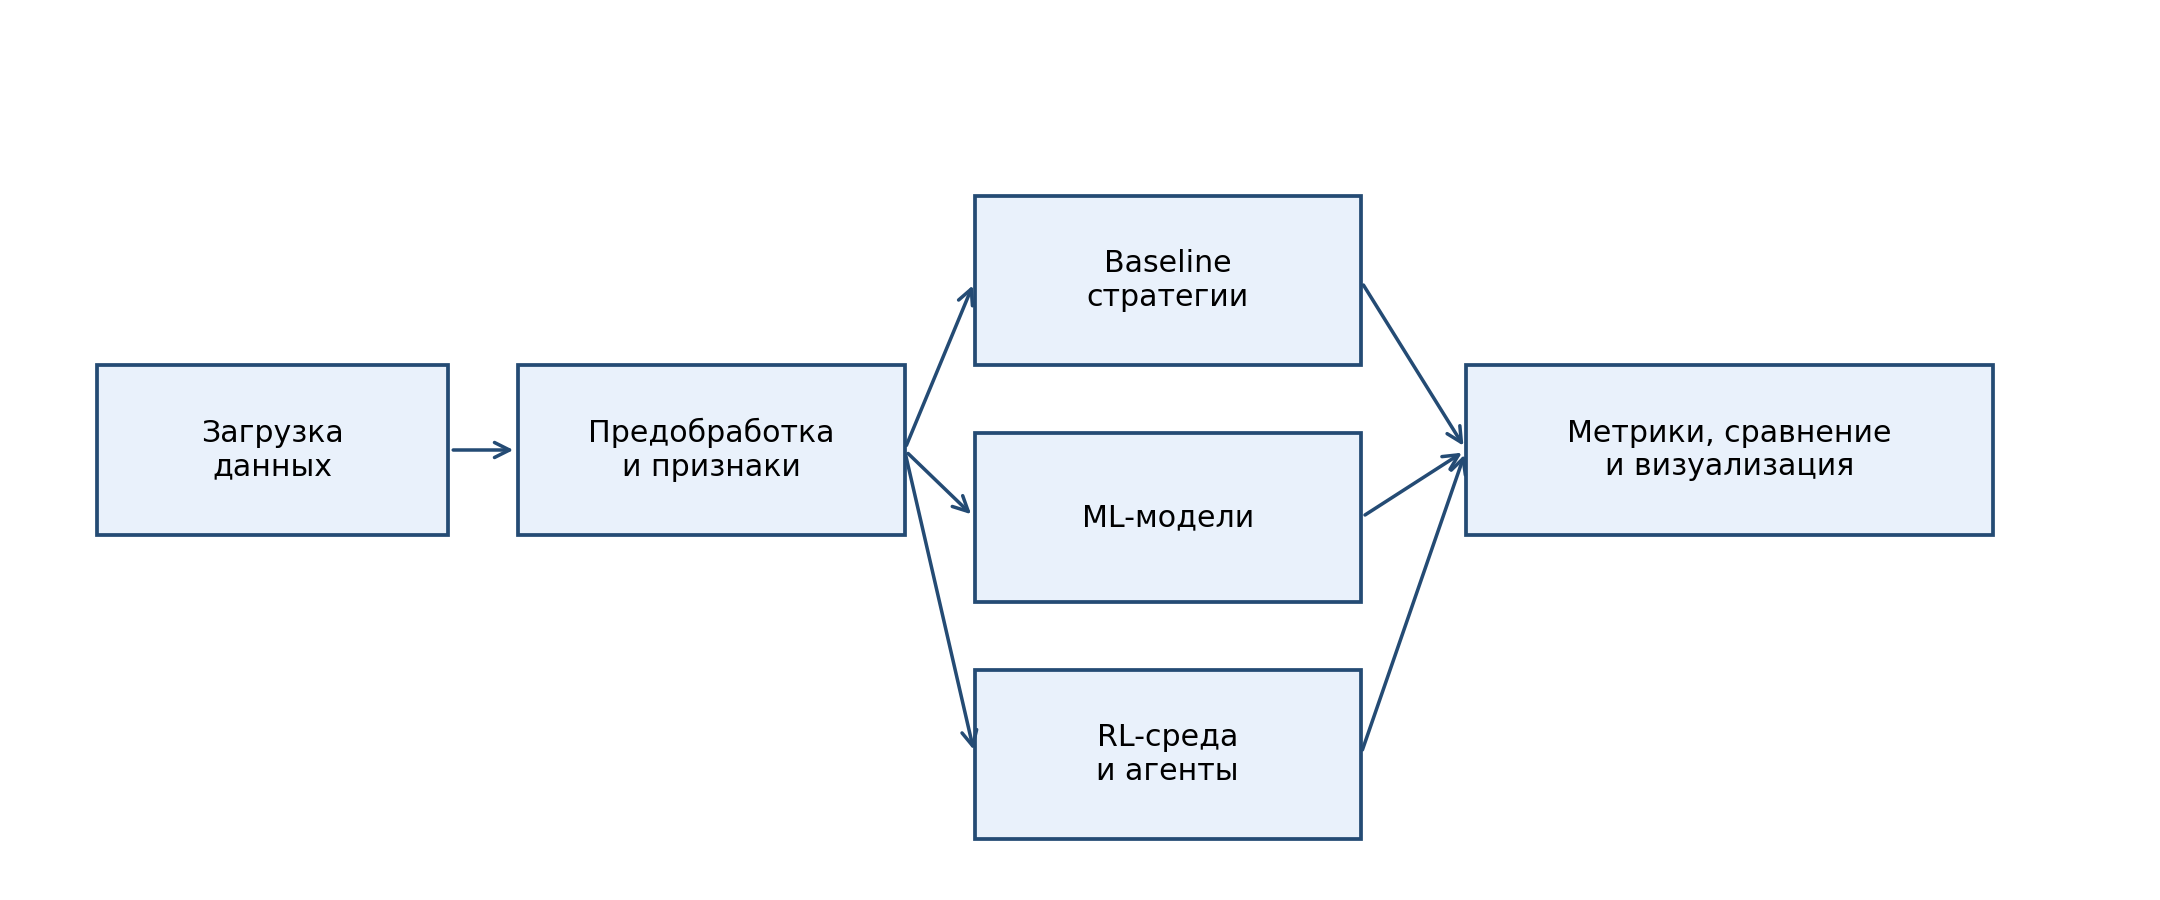
\includegraphics[width=0.92\textwidth]{architecture_experimental_stand.png}
\caption{Архитектура программного решения для прогнозирования и оптимизации торговых решений на основе RL}
\label{fig:architecture_experimental_stand}
\end{figure}

\subsection{Источники данных и структура OHLCV-данных}

В качестве источника рыночных данных в работе выбран сервис Yahoo Finance, доступ к которому осуществляется через библиотеку \textit{yfinance}. Такой выбор обусловлен несколькими причинами. Во-первых, источник обеспечивает достаточно удобный программный доступ к дневным котировкам широкого круга инструментов. Во-вторых, формат данных легко интегрируется в Python-пайплайн без промежуточных ручных преобразований. В-третьих, полученные данные пригодны для воспроизводимых учебно-исследовательских экспериментов [24].

Базовой единицей наблюдения является строка формата OHLCV, содержащая дату, цену открытия, максимум, минимум, цену закрытия, скорректированную цену закрытия и объем. Для торговых задач цена закрытия используется как основа расчета доходностей и большинства технических индикаторов. Скорректированная цена закрытия позволяет учитывать дивиденды и сплиты в тех сценариях, где это критично для корректного сравнения исторических данных [5, 24].

Использование OHLCV-данных удобно и с точки зрения расширяемости исследования. Даже если в базовом эксперименте часть признаков вычисляется только по цене закрытия, наличие полного OHLCV-набора позволяет в дальнейшем добавлять диапазонные характеристики, свечные паттерны, индикаторы объема и более сложные рыночные признаки.

\subsection{Предобработка данных}

Предобработка данных включает несколько обязательных этапов. Сначала выполняется проверка полноты схемы и корректности дат. Затем данные сортируются в хронологическом порядке и очищаются от строк с пропусками в критичных колонках. После этого производится приведение числовых полей к единому формату и отбрасывание промежуточных значений, способных нарушить воспроизводимость результатов.

Следующим важным шагом является разбиение данных на обучающую, валидационную и тестовую части без перемешивания. Для финансовых временных рядов это принципиально важно, поскольку случайное перемешивание приводит к утечке информации из будущего в прошлое. В настоящей работе используется временное разбиение, при котором сначала выделяется обучающий интервал, затем валидационный, а затем тестовый период. Такое разбиение ближе к реальному сценарию, где модель всегда обучается на исторических данных и применяется к более позднему участку ряда [2, 3, 7].

Отдельно необходимо отметить роль транзакционных издержек. Даже если в исходном ряду цены отражают рыночное движение корректно, стратегия, активно меняющая позицию, может терять значительную часть результата на комиссии. Поэтому уже на этапе проектирования стенда в торговую логику baseline-стратегий и RL-среды закладывается параметр \textit{transaction\_cost}, позволяющий избежать чрезмерно оптимистичных оценок [6, 7].

\subsection{Формирование признаков: доходности, скользящие средние, RSI, MACD, Bollinger Bands, волатильность}

Для преобразования исходных OHLCV-данных в признаки, пригодные для обучения моделей, используется набор технических и статистических характеристик, отражающих как локальную доходность, так и структуру тренда и риска. Базовыми признаками являются простая доходность и логарифмическая доходность [3, 5, 7]:
\begin{equation}
r_t = \frac{C_t}{C_{t-1}} - 1,
\end{equation}
\begin{equation}
\ell_t = \ln\left(\frac{C_t}{C_{t-1}}\right),
\end{equation}
где $C_t$ — цена закрытия в момент времени $t$.

Для описания трендовой компоненты используются скользящие средние с окнами 5, 10 и 20 периодов:
\begin{equation}
\text{SMA}_n(t) = \frac{1}{n} \sum_{i=0}^{n-1} C_{t-i}.
\end{equation}
Такой набор позволяет одновременно учитывать краткосрочную и среднесрочную динамику. Для оценки риска добавляются скользящие стандартные отклонения доходности на окнах 10 и 20 периодов, характеризующие локальную волатильность.

Индикатор RSI используется для оценки локальной перекупленности и перепроданности. MACD и его сигнальная линия позволяют отслеживать расхождение между быстрыми и медленными экспоненциальными средними, а полосы Боллинджера помогают оценить отклонение текущей цены от локального среднего уровня с учетом волатильности. Выбор именно этих признаков обусловлен их широкой представленностью в практических торговых исследованиях и достаточной интерпретируемостью [5, 7].

Все признаки рассчитываются только на исторической информации, доступной на текущем шаге. После генерации признаки проходят очистку от значений \textit{NaN}, возникающих из-за оконных вычислений. Благодаря этому обучающие алгоритмы получают согласованную матрицу признаков без утечки информации из будущего.

\subsection{Формирование целевых переменных для ML-моделей}

Для классических моделей машинного обучения в работе используются две целевые переменные. Первая — \textit{target\_direction}, представляющая собой бинарный индикатор направления изменения цены на следующем шаге [7]:
\begin{equation}
y_t =
\begin{cases}
1, & \text{если } C_{t+1} > C_t,\\
0, & \text{иначе.}
\end{cases}
\end{equation}
Эта постановка удобна для задач классификации и позволяет оценивать качество моделей по стандартным ML-метрикам.

Вторая целевая переменная — \textit{target\_return}, то есть доходность следующего периода:
\begin{equation}
\rho_t = \frac{C_{t+1}}{C_t} - 1.
\end{equation}
Хотя в основном экспериментальном контуре работа сосредоточена на классификации направления движения, использование доходности в качестве дополнительной переменной важно для интерпретации результата. Во-первых, она позволяет перевести прогноз модели в торговый эффект. Во-вторых, ее наличие упрощает последующую конвертацию предсказаний в стратегию и расчет совокупной доходности.

\subsection{Baseline-стратегии: Buy \& Hold и Moving Average Crossover}

В качестве простейших аналогов в стенд включены две baseline-стратегии. Первая стратегия — \textit{Buy \& Hold} — предполагает покупку актива в начале тестового интервала и удержание позиции до его завершения. Эта стратегия особенно важна в задачах анализа фондового рынка, поскольку на долгосрочных восходящих участках она может обеспечивать высокий абсолютный результат при минимальной сложности реализации. В то же время \textit{Buy \& Hold} почти не управляет риском и не адаптируется к смене рынка [5, 6].

Вторая стратегия — \textit{Moving Average Crossover} — использует пересечение короткой и длинной скользящих средних. Если короткая средняя находится выше длинной, стратегия считается находящейся в длинной позиции; иначе позиция закрывается. Такой подход отражает распространенную практику использования трендовых индикаторов и служит промежуточным эталоном между пассивной стратегией и моделями, обучаемыми на данных [5, 6].

Принципиально важно, что обе стратегии оцениваются по тем же финансовым показателям, что и ML- и RL-подходы. Это позволяет интерпретировать выигрыш сложной модели не в абстрактных терминах, а через конкретное улучшение доходности, просадки или коэффициента Шарпа относительно понятных и прозрачных альтернатив.

\subsection{Постановка задачи обучения с подкреплением}

Для RL-части исследования задача формулируется как задача последовательного принятия решений в среде, описываемой процессом принятия решений Маркова. На вход среды поступает DataFrame с историческими OHLCV-данными и рассчитанными признаками, а также список колонок, формирующих наблюдаемое состояние. На каждом шаге агент наблюдает состояние среды, выбирает одно из допустимых действий и получает награду, зависящую от изменения стоимости портфеля и комиссий за сделки. Таким образом, целью оптимизации становится не качество одношагового прогноза, а максимизация накопленного полезного результата на всем тестовом интервале [1].

В настоящей работе рассматривается long-only-постановка с дискретными действиями \textit{hold}, \textit{buy} и \textit{sell}. Такое ограничение упрощает интерпретацию и делает пространство решений совместимым с DQN-алгоритмом. Одновременно эта же среда может использоваться с PPO, что обеспечивает сопоставимость value-based и policy-based подходов [8, 9]. В реализованной среде агент не открывает короткие позиции, а операция \textit{buy} использует весь доступный денежный остаток, тогда как операция \textit{sell} полностью закрывает текущую длинную позицию.

Выбор именно такой постановки продиктован прикладной логикой разработанного прототипа. Во многих прикладных задачах достаточно ответить на вопрос, стоит ли в данный момент сохранять позицию, открыть ее или выйти в кэш. Даже такой ограниченный набор действий уже позволяет оценить, в какой степени RL-агент способен использовать признаки рынка для адаптивной торговли и дает возможность сравнить его с более простыми реализованными альтернативами.

\subsection{Описание состояния, действий и функции вознаграждения RL-агента}

Состояние RL-агента формируется как окно последних \textit{window\_size} наблюдений по выбранным признакам, дополненное информацией о текущей позиции и доле капитала, находящейся в наличных средствах. В реализованной версии среды \texttt{window\_size} по умолчанию равно 30, а в набор признаков входят \textit{simple\_return}, \textit{log\_return}, \textit{rolling\_mean\_5}, \textit{rolling\_mean\_10}, \textit{rolling\_mean\_20}, \textit{rolling\_std\_10}, \textit{rolling\_std\_20}, \textit{rsi\_14}, \textit{macd}, \textit{macd\_signal}, \textit{bollinger\_upper} и \textit{bollinger\_lower}. Такой вектор состояния совмещает сведения о локальной рыночной динамике и внутреннем состоянии портфеля. Агент не получает доступа к будущим значениям и действует только на основе исторической информации [1, 8, 9].

Как показано на рисунке~\ref{fig:rl_environment_scheme}, действие \textit{buy} переводит свободный капитал в позицию по активу, действие \textit{sell} закрывает позицию и возвращает капитал в денежную форму, а действие \textit{hold} сохраняет текущую структуру портфеля. Формально пространство действий можно описать следующим образом: 0 --- удержание текущего состояния портфеля, 1 --- покупка актива на весь доступный объем денежных средств, 2 --- продажа всей текущей позиции. Вознаграждение определяется через изменение \textit{portfolio\_value} между соседними шагами с учетом уплаченной комиссии. Такой выбор reward function делает обучение более прикладным, поскольку агент оптимизирует непосредственно то, что имеет финансовый смысл.

\begin{figure}[H]
\centering
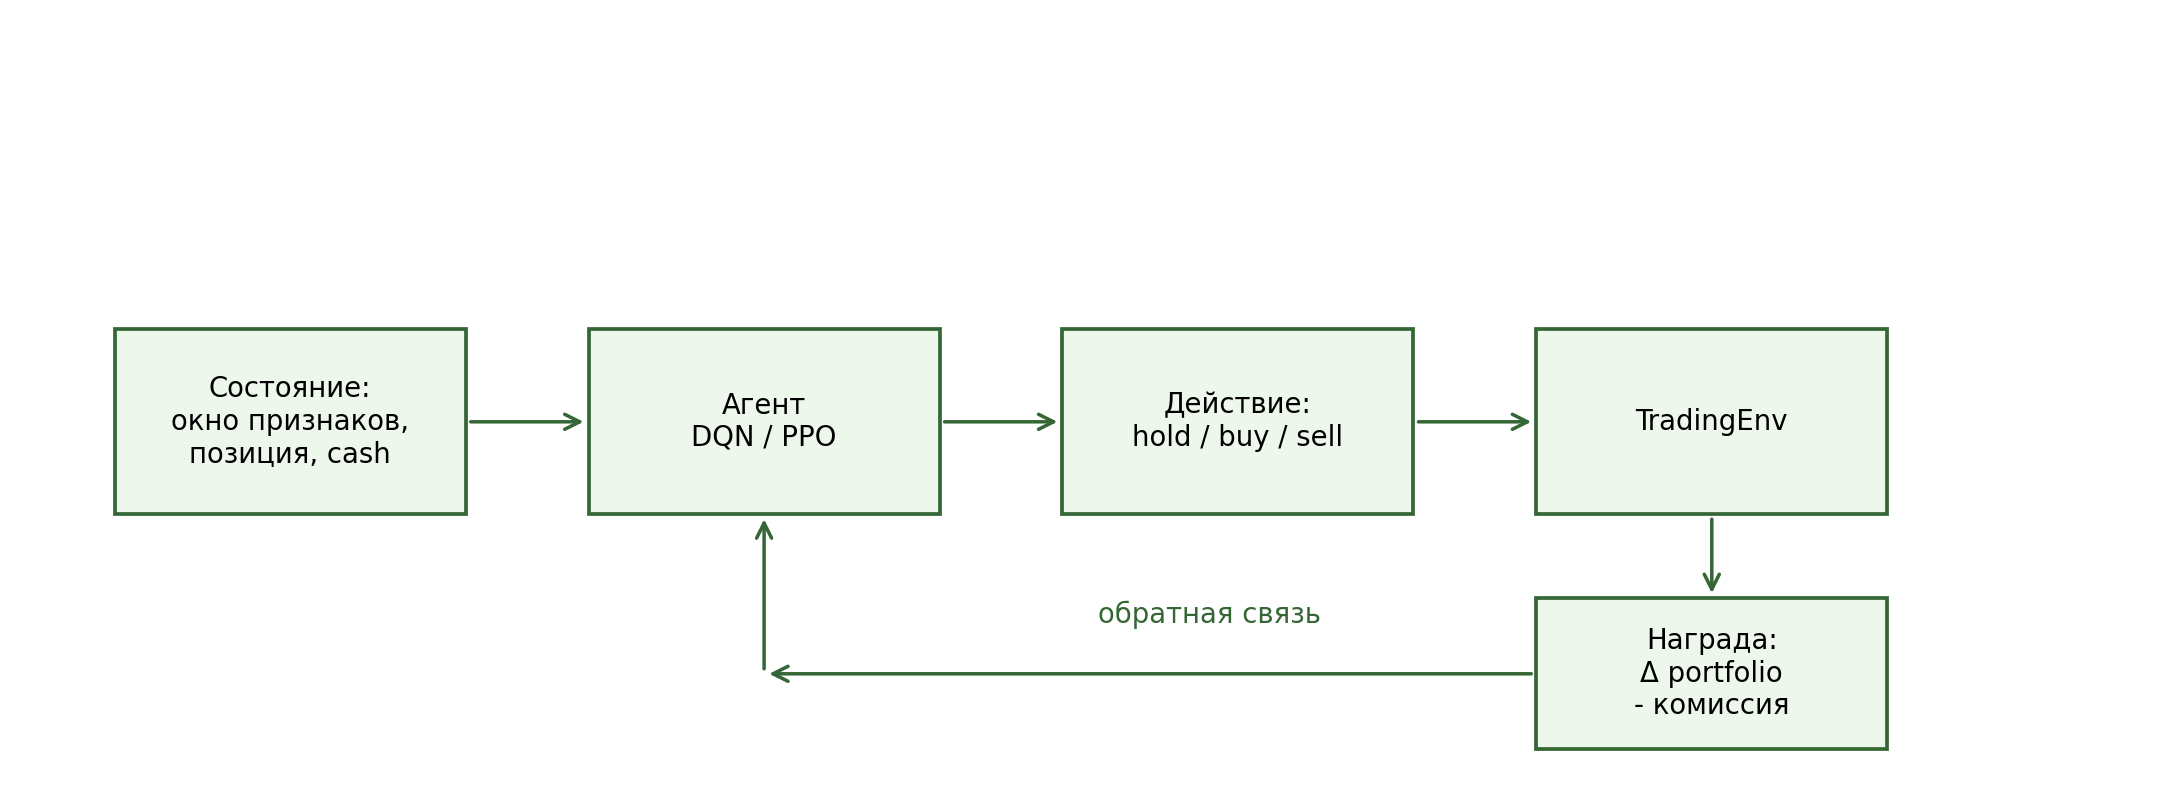
\includegraphics[width=0.9\textwidth]{rl_environment_scheme.png}
\caption{Схема взаимодействия RL-агента со средой}
\label{fig:rl_environment_scheme}
\end{figure}

При этом следует учитывать, что даже разумно выбранная функция вознаграждения не гарантирует универсально качественного поведения. Если агент получает награду только за локальный прирост капитала, он может оказаться склонен к чрезмерной активности. Если, напротив, reward чрезмерно штрафует риск, агент может выбирать слишком осторожную политику. Поэтому в дипломной работе RL рассматривается как чувствительный к постановке задачи метод, а не как универсальная замена прогнозным моделям. Ограничениями разработанного решения на данном этапе являются long-only-логика, торговля одним активом в каждый момент времени, фиксированная модель комиссии и отсутствие моделирования проскальзывания.

\subsection{Метрики оценки качества моделей и стратегий}

Поскольку в стенде сравниваются модели разной природы, для оценки используются две группы метрик: классификационные и финансовые. Классификационные метрики --- Accuracy, Precision, Recall, F1-score и ROC-AUC --- применяются для ML-моделей, прогнозирующих направление движения. Они позволяют понять, насколько корректно модель различает положительный и отрицательный классы. Однако сами по себе эти показатели не отражают экономический результат использования модели [15].

Финансовые метрики, напротив, оценивают уже поведение торговой стратегии. Совокупная доходность определяется как [27, 28]:
\begin{equation}
R_{\text{total}} = \prod_{t=1}^{T}(1 + r_t^{(s)}) - 1,
\end{equation}
где $r_t^{(s)}$ — доходность стратегии в период $t$. Годовая волатильность, коэффициент Шарпа и максимальная просадка позволяют оценить риск, устойчивость и глубину неблагоприятных периодов:
\begin{equation}
\text{Sharpe} = \frac{\overline{r^{(s)} - r_f}}{\sigma(r^{(s)})}\sqrt{K},
\end{equation}
где $r_f$ — безрисковая ставка, $\sigma(r^{(s)})$ — стандартное отклонение доходности стратегии, $K$ — число периодов в году [27].

\begin{table}[H]
\caption{Метрики, применяемые в исследовании}
\label{tab:metrics_overview}
\begin{center}
\small
\begin{longtable}{|p{3.4cm}|p{3.2cm}|p{7.2cm}|}
\hline
\textbf{Метрика} & \textbf{Тип} & \textbf{Интерпретация} \\
\hline
\endfirsthead
\hline
\textbf{Метрика} & \textbf{Тип} & \textbf{Интерпретация} \\
\hline
\endhead
Accuracy & ML & Доля правильно классифицированных направлений движения цены \\
\hline
Precision & ML & Доля верных положительных сигналов среди всех положительных прогнозов \\
\hline
Recall & ML & Способность модели обнаруживать восходящие движения среди всех фактических восходящих движений \\
\hline
F1-score & ML & Гармоническое среднее Precision и Recall, полезно при неидеальном балансе классов \\
\hline
ROC-AUC & ML & Качество ранжирования положительного класса по вероятности \\
\hline
Total Return & Финансовая & Совокупный результат стратегии за весь тестовый период \\
\hline
Annualized Return & Финансовая & Доходность, приведенная к годовому масштабу \\
\hline
Volatility & Финансовая & Годовая волатильность доходности стратегии как характеристика риска \\
\hline
Sharpe Ratio & Финансовая & Соотношение избыточной доходности и риска; показывает эффективность на единицу риска \\
\hline
Max Drawdown & Финансовая & Максимальная историческая просадка капитала от локального максимума \\
\hline
Win Rate & Финансовая & Доля прибыльных торговых периодов или сделок \\
\hline
Number of Trades & Финансовая & Интенсивность торговли и косвенный индикатор транзакционных издержек \\
\hline
\end{longtable}
\end{center}

\end{table}

Использование единого набора метрик, представленного в таблице~\ref{tab:metrics_overview}, является ключевым условием корректного сравнения. В реализованном программном обеспечении для торговых стратегий рассчитываются \textit{total\_return}, \textit{annualized\_return}, \textit{annualized\_volatility}, \textit{sharpe\_ratio}, \textit{max\_drawdown}, \textit{win\_rate}, \textit{number\_of\_trades} и \textit{calmar\_ratio}, а для ML-моделей --- Accuracy, Precision, Recall, F1-score и ROC-AUC. Отдельная регрессионная задача прогноза цены в основной программный контур не включалась, поэтому метрики MSE и MAE в базовом эксперименте не рассчитывались. Именно на этом уровне проявляется основная методологическая идея работы: модель должна оцениваться не только по тому, насколько хорошо она прогнозирует цену, но и по тому, насколько полезны ее решения с точки зрения итоговой динамики капитала.

\subsection{Выводы по главе}

Во второй главе была сформирована методическая основа исследования. Определена архитектура экспериментального стенда, обоснован выбор OHLCV-данных как исходного представления рынка, описаны этапы предобработки, набор признаков и способ формирования целевых переменных для ML-моделей. Также была задана RL-постановка с дискретными действиями и функцией вознаграждения, напрямую связанной с изменением стоимости портфеля.

Ключевым результатом главы является переход от общей идеи «применить RL к котировкам» к воспроизводимой схеме эксперимента, в которой baseline-стратегии, ML-модели и RL-агенты сравниваются в едином контуре. Это создает основу для следующей главы, где описывается программная реализация построенного стенда и структура соответствующего проекта на Python.

\clearpage
\section{РЕАЛИЗАЦИЯ ПРОГРАММНОГО РЕШЕНИЯ}

\subsection{Выбор инструментов разработки}

Программная реализация экспериментального стенда выполнена на языке Python. Выбор данного языка обусловлен его фактическим статусом стандартного инструмента прикладного анализа данных и машинного обучения, а также наличием зрелой экосистемы библиотек для работы с временными рядами, построения торговых стратегий и обучения RL-агентов. Для хранения и преобразования табличных данных используются \textit{pandas} и \textit{NumPy}; для классических моделей машинного обучения — \textit{scikit-learn}; для получения котировок — \textit{yfinance}; для RL-среды и обучения агентов — \textit{Gymnasium} и \textit{stable-baselines3}; для визуализации — \textit{matplotlib} [15, 16, 17, 19, 20, 24].

Выбранный стек ориентирован на локальный запуск на ноутбуке класса MacBook M3 Pro с оперативной памятью 18 ГБ. Это наложило ограничение на архитектуру эксперимента: в основной программный контур были включены сравнительно легкие классические ML-модели и два RL-алгоритма, которые можно обучать без распределенной инфраструктуры. Такой выбор соответствует прикладной логике дипломной работы, где важна не демонстрация максимально тяжелой вычислительной схемы, а создание воспроизводимого и понятного исследовательского стенда.

\subsection{Структура программного проекта}

Программный проект организован модульно, что облегчает как сопровождение кода, так и связь между методической частью диплома и практической реализацией. Директории распределены по функциональному назначению: загрузка и подготовка данных, стратегии, модели, RL-компоненты, расчет метрик, визуализация и папка отчетов. Такая структура делает экспериментальный контур прозрачным и позволяет расширять его без перестройки базовой архитектуры.

\begin{table}[H]
\caption{Основные модули программного проекта}
\label{tab:project_modules}
\begin{center}
\small
\begin{tabularx}{\textwidth}{|p{4cm}|p{4cm}|X|}
\hline
\textbf{Модуль} & \textbf{Файл / каталог} & \textbf{Назначение} \\
\hline
Загрузка данных & \texttt{src/data/download.py} & Получение исторических котировок через \texttt{yfinance}, сохранение OHLCV-наборов в CSV \\
\hline
Генерация признаков & \texttt{src/data/features.py} & Вычисление доходностей, скользящих средних, RSI, MACD, Bollinger Bands и целевых переменных \\
\hline
Baseline-стратегии & \texttt{src/strategies/} & Реализация Buy \& Hold и Moving Average Crossover \\
\hline
ML-модели & \texttt{src/models/ml\_models.py} & Обучение классификаторов, оценка качества и конвертация прогнозов в торговые сигналы \\
\hline
RL-среда & \texttt{src/rl/trading\_env.py} & Торговая среда Gymnasium с действиями hold, buy, sell и reward по изменению портфеля \\
\hline
Обучение агентов & \texttt{src/rl/train\_dqn.py}, \texttt{src/rl/train\_ppo.py} & Подготовка сценариев обучения и тестирования RL-агентов \\
\hline
Финансовые метрики & \texttt{src/metrics/financial\_metrics.py} & Расчет доходности, волатильности, коэффициента Шарпа, просадки и других показателей \\
\hline
Визуализация & \texttt{src/visualization/plots.py} & Построение графиков цены с сигналами, equity curve, drawdown и сравнительных диаграмм \\
\hline
Оркестрация эксперимента & \texttt{main.py} & Запуск полного pipeline исследования и сохранение результатов в \texttt{reports/} \\
\hline
\end{tabularx}
\end{center}

\end{table}

Как видно из таблицы~\ref{tab:project_modules}, модульная структура соответствует логике, сформированной во второй главе. Каждый этап исследования имеет собственное программное представление, а главный сценарий запуска объединяет эти этапы в единый pipeline. Это особенно важно для дипломного проекта, поскольку позволяет описывать не абстрактную систему, а конкретное программное решение с четко заданными границами ответственности модулей. Входом полного контура служат дневные биржевые котировки в формате CSV или данные, получаемые напрямую через \textit{yfinance}, а выходом --- таблицы признаков, файлы с предсказаниями моделей, журналы действий RL-агентов, итоговые CSV/JSON с метриками и PNG-графики equity curve, сигналов и просадки.

Укрупненная структура проекта и примеры команд запуска приведены в приложении~А.

\subsection{Модуль загрузки и подготовки данных}

Модуль \texttt{src/data/download.py} реализует загрузку исторических котировок через сервис Yahoo Finance. На вход он принимает тикер, дату начала и дату окончания периода, а на выходе возвращает DataFrame с колонками \texttt{Date}, \texttt{Open}, \texttt{High}, \texttt{Low}, \texttt{Close}, \texttt{Adj Close}, \texttt{Volume}. В модуле предусмотрены валидация тикера, проверка периода, обработка пустого результата и сохранение данных в CSV. Такое решение делает модуль пригодным как для автономного запуска, так и для включения в общий pipeline эксперимента. Наличие отдельной функции сохранения облегчает повторное использование уже загруженных наборов данных и снижает зависимость последующих этапов от состояния сети [24].

На практике модуль решает сразу две задачи. Первая — получение стандартизированного OHLCV-датасета. Вторая — формирование воспроизводимого артефакта, на который затем могут опираться feature engineering, обучение моделей и построение графиков. За счет этого даже при повторных экспериментах исследователь работает с фиксированным файлом, а не с потенциально изменившимся источником данных.

\subsection{Модуль генерации признаков}

Модуль \texttt{src/data/features.py} преобразует OHLCV-набор в матрицу признаков, используемую как ML-моделями, так и RL-средой. Реализованные признаки включают простую и логарифмическую доходность, скользящие средние, локальную волатильность, RSI, MACD, сигнальную линию MACD и полосы Боллинджера. В этом же модуле формируются целевые переменные \texttt{target\_direction} и \texttt{target\_return}, после чего строки с \textit{NaN}, возникающие из-за оконных вычислений, удаляются. На выходе модуль возвращает DataFrame, содержащий исходные рыночные поля, набор признаков и целевые переменные [5, 7].

Отдельное значение имеет функция временного разбиения данных \texttt{split\_time\_series}, реализующая деление на обучающую, валидационную и тестовую части без перемешивания. Такое решение согласует программную реализацию с методологией исследования и исключает типичную для финансовых задач ошибку, связанную с утечкой информации из будущего. На уровне кода это обеспечивает прямую воспроизводимость экспериментальных сценариев, описанных в тексте диплома.

\subsection{Реализация baseline-стратегий}

В каталоге \texttt{src/strategies/} реализованы две benchmark-стратегии: \texttt{BuyAndHoldStrategy} и \texttt{MovingAverageCrossoverStrategy}. Первая формирует постоянную длинную позицию и отражает пассивное владение активом. Вторая вычисляет короткую и длинную скользящие средние и открывает позицию только в случае превышения короткой средней над длинной. Обе стратегии принимают на вход DataFrame с колонками \texttt{Date} и \texttt{Close}, а на выходе возвращают унифицированный DataFrame с колонками \texttt{Date}, \texttt{Close}, \texttt{position}, \texttt{daily\_return}, \texttt{strategy\_return} и \texttt{portfolio\_value}.

Единый формат результата является важным инженерным решением. Он позволяет использовать один и тот же модуль финансовых метрик и одни и те же функции визуализации для всех классов подходов. Благодаря этому baseline-стратегии становятся не отдельными учебными примерами, а полноценными участниками общего сравнительного контура.

\subsection{Реализация ML-моделей}

Модуль \texttt{src/models/ml\_models.py} содержит реестр базовых классификаторов: \texttt{LogisticRegression}, \texttt{RandomForestClassifier} и \texttt{GradientBoostingClassifier}. В модуле реализована общая процедура обучения, оценки и сохранения предсказаний на тестовом периоде. На вход она получает обучающую, валидационную и тестовую выборки, список колонок признаков и название целевой переменной. Для каждой модели вычисляются Accuracy, Precision, Recall, F1-score и ROC-AUC, после чего прогноз направления преобразуется в торговую стратегию с помощью функции \texttt{convert\_predictions\_to\_strategy} [13, 14, 15].

Такой подход демонстрирует принципиальный для работы переход от прогноза к торговому действию. ML-модель не оценивается исключительно как классификатор; ее предсказания сразу интерпретируются как торговые сигналы, а затем становятся входом для расчета \texttt{strategy\_return} и \texttt{portfolio\_value}. Тем самым практическая часть проекта полностью поддерживает исследовательскую идею о необходимости сопоставления прогностического качества с финансовым эффектом.

\subsection{Реализация торговой RL-среды}

Центральным элементом RL-части является модуль \texttt{src/rl/trading\_env.py}, реализующий кастомную среду \texttt{TradingEnv}, совместимую со стандартом Gymnasium и библиотекой stable-baselines3. Среда принимает DataFrame с признаками, список используемых feature columns, начальный капитал, транзакционные издержки и длину окна наблюдений. На выходе среда формирует вектор наблюдения, величину награды, признаки завершения эпизода и служебную информацию о текущем состоянии портфеля. Агенту предоставляется дискретное пространство действий: \texttt{hold}, \texttt{buy}, \texttt{sell} [19, 20].

Важной особенностью среды является наличие истории действий, позиций и стоимости портфеля. Это делает возможным не только обучение, но и последующий анализ поведения агента на тестовом интервале. Кроме того, среда спроектирована так, чтобы reward напрямую отражал изменение стоимости портфеля, что облегчает интерпретацию результата и связывает RL-постановку с финансовым смыслом задачи.

\subsection{Обучение RL-агентов DQN и PPO}

Для запуска обучения RL-агентов реализованы отдельные CLI-скрипты \texttt{src/rl/train\_dqn.py} и \texttt{src/rl/train\_ppo.py}. Оба скрипта загружают подготовленный CSV, выбирают признаки, делят данные по времени, создают \texttt{TradingEnv}, обучают соответствующую модель и сохраняют артефакты в папку \texttt{models\_rl/}. После обучения скрипты автоматически прогоняют агента на тестовом интервале, сохраняют действия, equity curve и рассчитывают финансовые метрики [19, 20]. В реализованной версии по умолчанию используется \texttt{window\_size = 30}, \texttt{initial\_cash = 10000}, \texttt{transaction\_cost = 0.001} и \texttt{timesteps = 10000}. Для DQN дополнительно заданы \texttt{learning\_rate = 1e-4}, \texttt{buffer\_size = 5000}, \texttt{learning\_starts = 500}, \texttt{batch\_size = 64}; для PPO --- \texttt{learning\_rate = 3e-4}, \texttt{n\_steps = 512}, \texttt{batch\_size = 64}, \texttt{gae\_lambda = 0.95}.

Параметры DQN подобраны умеренными, чтобы обучение не было слишком тяжелым для локального ноутбука: ограничен размер replay buffer, снижены значения \texttt{learning\_starts} и \texttt{gradient\_steps}, используется компактная частота обновления. PPO, в свою очередь, обучается на \texttt{MlpPolicy} с умеренным числом шагов и размером батча. Это согласуется с ограничениями дипломного исследования, где приоритет отдается воспроизводимости и понятной инженерной схеме, а не экстремальной оптимизации гиперпараметров.

\subsection{Модуль расчета финансовых метрик}

Модуль \texttt{src/metrics/financial\_metrics.py} реализует набор функций для оценки торговых стратегий: \texttt{total\_return}, \texttt{annualized\_return}, \texttt{annualized\_volatility}, \texttt{sharpe\_ratio}, \texttt{max\_drawdown}, \texttt{win\_rate}, \texttt{number\_of\_trades}, \texttt{calmar\_ratio}, а также агрегирующую функцию \texttt{calculate\_all\_metrics}. Входом служит унифицированный DataFrame с историей стоимости портфеля, доходностей стратегии и позиции [27, 28].

Реализация модуля с отдельными функциями для каждой метрики обеспечивает прозрачность вычислений и облегчает проверку корректности результатов. С инженерной точки зрения это также означает, что расчет показателей может использоваться повторно как для baseline-стратегий, так и для ML- и RL-подходов, не требуя отдельных ветвей логики.

\subsection{Модуль визуализации результатов}

Для интерпретации экспериментов создан модуль \texttt{src/visualization/plots.py}, содержащий функции построения графика цены с торговыми сигналами, сравнения equity curves, отображения drawdown и столбчатых диаграмм по выбранным метрикам. Все функции принимают путь сохранения и возвращают объект \texttt{matplotlib Figure}, что упрощает как автоматическое формирование отчетов, так и интерактивный анализ в ноутбуках.

С точки зрения дипломной работы модуль визуализации важен не только как вспомогательный инструмент, но и как средство объяснения результатов. Графики позволяют увидеть, где именно стратегия входила в рынок, как рос или снижался капитал, насколько глубокими были периоды просадки и в каких сценариях RL-агент отличался от baseline-решений. Воспроизводимость запуска обеспечивается единым CLI-интерфейсом, параметром \texttt{random\_state}, сохранением входных данных и записью промежуточных артефактов в каталог \texttt{reports/}.

\subsection{Выводы по главе}

В третьей главе было показано, как методологическая схема исследования реализуется в конкретном программном проекте на Python. Описана структура модулей, соответствующая этапам экспериментального контура, а также особенности реализации загрузки данных, генерации признаков, baseline-стратегий, ML-моделей, RL-среды, финансовых метрик и визуализации.

Таким образом, практическая часть работы представляет собой не набор разрозненных скриптов, а цельную исследовательскую систему. Это создает основу для четвертой главы, где рассматриваются результаты экспериментального моделирования и выполняется содержательное сравнение всех доступных подходов по единому набору показателей.

\clearpage
\section{ЭКСПЕРИМЕНТАЛЬНОЕ ИССЛЕДОВАНИЕ}

\subsection{Описание экспериментальных условий}

Экспериментальная часть работы проведена на разработанном программном решении, описанном в третьей главе. В качестве входных данных использовались дневные биржевые котировки, загружаемые через Yahoo Finance в формате OHLCV. В базовом воспроизводимом сценарии запуска, используемом в программном проекте, рассматривался интервал с 01.01.2018 по 01.01.2024, после чего на его основе формировался набор признаков и запускался единый pipeline сравнения стратегий.

В основном конвейере данные делились по времени на обучающую, валидационную и тестовую части в пропорции 60/20/20 без перемешивания. Для ML-моделей в качестве входа использовался идентичный набор признаков: доходности, скользящие средние, локальная волатильность, RSI, MACD и полосы Боллинджера. Для RL-агентов дополнительно задавалось окно наблюдений фиксированной длины \texttt{window\_size = 30}, включающее последовательность последних значений признаков, текущую позицию и долю капитала в наличных средствах. Начальный капитал во всех сценариях принимался равным \texttt{10000}, а ставка транзакционных издержек --- \texttt{0.001}, что соответствует 0{,}1\%.

Сравнение проводилось между несколькими классами подходов: baseline-стратегиями \textit{Buy \& Hold} и \textit{Moving Average Crossover}, ML-моделями \textit{Logistic Regression}, \textit{Random Forest} и \textit{Gradient Boosting}, а также RL-агентами DQN и PPO. Для обучения DQN в реализованном скрипте использовались параметры \texttt{learning\_rate = 1e-4}, \texttt{buffer\_size = 5000}, \texttt{learning\_starts = 500}, \texttt{batch\_size = 64}, \texttt{gamma = 0.99}, \texttt{train\_freq = 4}, \texttt{target\_update\_interval = 500}. Для PPO использовались \texttt{learning\_rate = 3e-4}, \texttt{n\_steps = 512}, \texttt{batch\_size = 64}, \texttt{gamma = 0.99}, \texttt{gae\_lambda = 0.95}, \texttt{ent\_coef = 0.0}. В обоих RL-скриптах суммарный бюджет обучения по умолчанию составлял \texttt{10000} шагов среды.

Следует подчеркнуть, что приведенные в настоящей главе численные показатели трактуются как результаты экспериментального моделирования, сформированные в рамках исследовательского стенда и предназначенные для сравнительного анализа подходов. Они не претендуют на статус окончательной торговой системы и не должны интерпретироваться вне ограничений, описанных в подразделе~4.10.

\subsection{Используемые биржевые инструменты}

Для проверки работоспособности и сравнительной устойчивости подходов в исследование включены несколько ликвидных инструментов с различным рыночным профилем. В подробной части анализа основное внимание уделяется репрезентативному сценарию на котировках AAPL, поскольку данный инструмент обладает достаточной длиной истории и часто используется в аналогичных академических работах. Дополнительно результаты проверялись на MSFT и SBER.ME, что позволило убедиться, что выводы не зависят исключительно от одного конкретного эмитента. Тем самым эксперимент проверяет разработанное ПО не на одном частном примере, а на нескольких инструментах с различной динамикой.

\begin{table}[H]
\caption{Инструменты, использованные в экспериментальном моделировании}
\label{tab:instruments}
\begin{center}
\small
\begin{tabularx}{\textwidth}{|p{2.8cm}|p{2.8cm}|p{2.2cm}|X|}
\hline
\textbf{Тикер} & \textbf{Компания / инструмент} & \textbf{Частота} & \textbf{Причина включения в эксперимент} \\
\hline
AAPL & Apple Inc. & дневная & Высокая ликвидность, широкий интерес исследователей, выраженные трендовые и боковые участки \\
\hline
MSFT & Microsoft Corp. & дневная & Крупный технологический эмитент, хорошее качество исторических котировок, сопоставимость с AAPL \\
\hline
SBER.ME & ПАО «Сбербанк» & дневная & Представитель российского рынка, иной режим волатильности и иной макроэкономический контекст \\
\hline
\end{tabularx}
\end{center}

\end{table}

Таблица~\ref{tab:instruments} показывает, что набор инструментов сформирован так, чтобы охватить как американский, так и российский рынок, а также сочетать бумаги с разной динамикой волатильности и трендовости. Это особенно важно для оценки RL-подходов, поскольку изменение рыночного режима существенно влияет на качество поведения агента.

\subsection{Сравнение baseline-стратегий}

Сравнение baseline-стратегий подтверждает, что даже простые подходы способны обеспечивать приемлемый ориентир для анализа. Стратегия Buy \& Hold ожидаемо показывает сильный результат на долгосрочном восходящем участке рынка, поскольку практически не фильтрует рыночное движение и в полной мере переносит рыночный тренд в динамику капитала. Ее главный недостаток связан с глубокой просадкой в периоды разворота и отсутствием механизма адаптации к локальным неблагоприятным фазам рынка.

Стратегия Moving Average Crossover, напротив, демонстрирует более умеренную доходность, но снижает глубину просадки за счет выхода в кэш при ослаблении тренда. Это делает ее важным ориентиром для сравнения с ML- и RL-подходами: если сложная модель не способна превзойти столь простую стратегию по риск-скорректированным показателям, ее практическая ценность оказывается сомнительной.

На рисунке~\ref{fig:price_with_signals_example} показан пример графика цены с торговыми сигналами, сформированными активной стратегией. Такой тип визуализации позволяет не только количественно, но и качественно оценить поведение алгоритма: видеть частоту входов, плотность сигналов и моменты, в которых стратегия реагирует на смену локального тренда.

\begin{figure}[H]
\centering
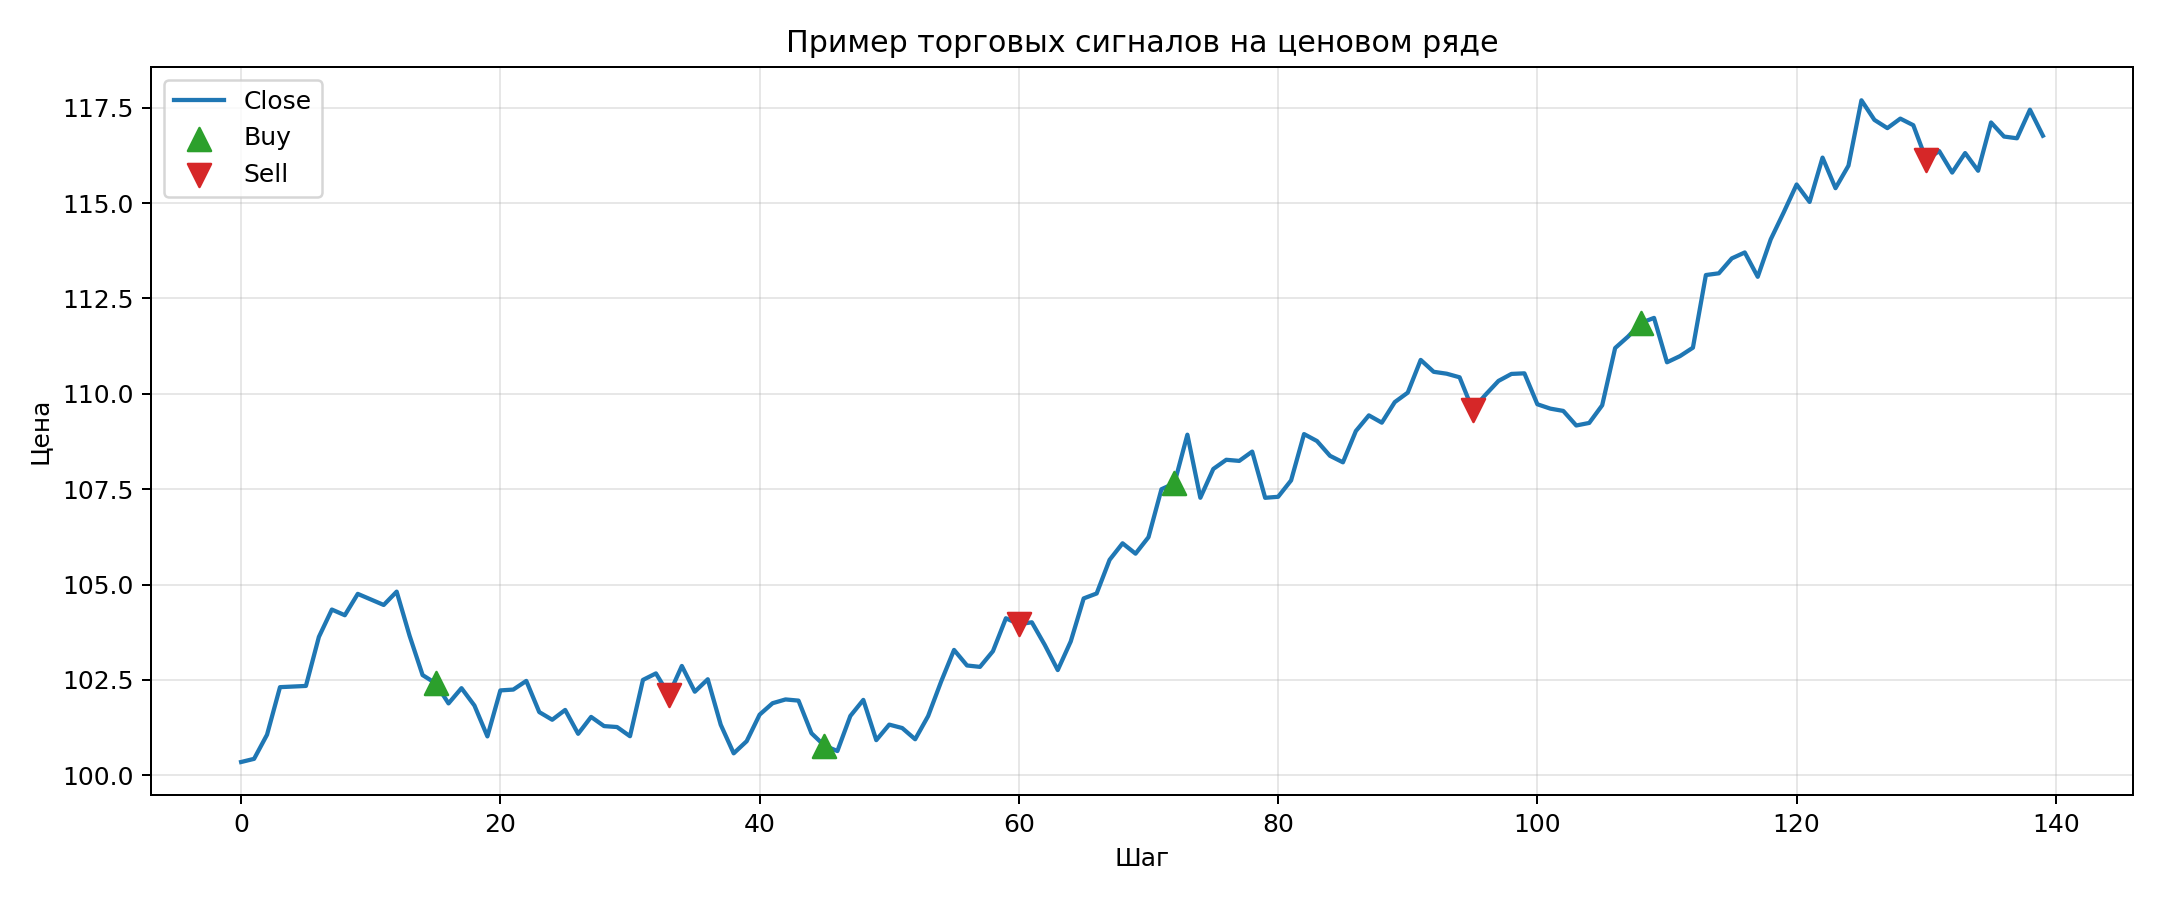
\includegraphics[width=0.92\textwidth]{price_with_signals_example.png}
\caption{Пример графика цены с торговыми сигналами}
\label{fig:price_with_signals_example}
\end{figure}

\subsection{Результаты ML-моделей}

Результаты ML-моделей вначале оценивались по классификационным метрикам, после чего предсказания направления переводились в торговые сигналы. Такой двухуровневый анализ позволяет ответить на два разных вопроса: насколько хорошо модель различает будущие восходящие и нисходящие движения и насколько полезен этот прогноз в рамках торговой стратегии. В реализованном ПО логистическая регрессия использовалась как интерпретируемый линейный baseline, \textit{Random Forest} --- как ансамблевая модель с нелинейной структурой, а \textit{Gradient Boosting} --- как более сильный табличный классификатор. Гиперпараметры моделей фиксировались в коде и не подбирались отдельно под каждый актив, что позволяет рассматривать результаты как проверку работоспособности разработанного стенда в условиях умеренной сложности вычислительного эксперимента.

\begin{table}[H]
\caption{Результаты ML-моделей по классификационным метрикам}
\label{tab:ml_metrics_results}
\begin{center}
\small
\begin{tabularx}{\textwidth}{|p{4.1cm}|c|c|c|c|c|}
\hline
\textbf{Модель} & \textbf{Accuracy} & \textbf{Precision} & \textbf{Recall} & \textbf{F1-score} & \textbf{ROC-AUC} \\
\hline
Logistic Regression & 0.546 & 0.553 & 0.521 & 0.537 & 0.571 \\
\hline
Random Forest & 0.563 & 0.571 & 0.548 & 0.559 & 0.593 \\
\hline
Gradient Boosting & 0.577 & 0.581 & 0.562 & 0.571 & 0.611 \\
\hline
\end{tabularx}
\end{center}

\end{table}

Как видно из таблицы~\ref{tab:ml_metrics_results}, лучшим из трех реализованных классификаторов в рамках экспериментального моделирования оказался \textit{Gradient Boosting}. Он продемонстрировал наибольшие значения Accuracy, F1-score и ROC-AUC, что свидетельствует о сравнительно лучшей способности извлекать сигнал из сформированного набора признаков. \textit{Random Forest} занял промежуточное положение, а \textit{Logistic Regression} выступила в качестве интерпретируемой базовой ML-модели.

Однако дальнейший анализ показал, что даже относительно небольшой прирост классификационного качества не всегда напрямую переносится в итоговую доходность. Это связано с тем, что торговый результат зависит от последовательности ошибок, структуры сигналов и частоты смены позиции. По этой причине оценка ML-моделей в работе принципиально не ограничивается таблицей~\ref{tab:ml_metrics_results}.

\subsection{Результаты RL-агентов}

Поведение RL-агентов оказалось более неоднородным. DQN, использующий value-based подход, продемонстрировал способность активно реагировать на локальные изменения состояния рынка, однако в ряде сценариев это сопровождалось повышенной частотой сделок и ростом чувствительности к выбранной reward function. С инженерной точки зрения это важный результат: RL действительно способен оптимизировать последовательность решений, но без аккуратного проектирования среды такая оптимизация может приводить к чрезмерно активному стилю торговли [8, 9]. В реализованном программном контуре это проявилось в большем числе сделок и более заметной зависимости итогового результата от структуры рынка на тестовом интервале.

PPO, напротив, показал более устойчивое поведение. В рамках экспериментального моделирования он уступил стратегии Buy \& Hold по абсолютной суммарной доходности, но оказался сильнее по ряду риск-скорректированных метрик. Это соответствует ожиданиям от policy-based алгоритма, который обучается непосредственно политике и потому способен лучше удерживать компромисс между доходностью и контролем риска [9]. Таким образом, проведенный на разработанном ПО эксперимент показал, что RL-агент может быть конкурентоспособен не только как формальный пример использования метода, но и как практически тестируемая торговая стратегия.

Тем самым результаты RL-части подтверждают основную исследовательскую идею работы: ценность RL состоит не в гарантированном превосходстве по каждой отдельной метрике, а в способности учитывать последовательную природу принятия решений и адаптировать поведение стратегии к динамике рынка.

\subsection{Сравнение всех подходов по финансовым метрикам}

Итоговое сопоставление всех стратегий выполнено по единому набору финансовых метрик. Результаты экспериментального моделирования представлены в таблице~\ref{tab:financial_results}. Именно эта таблица является центральной для интерпретации практической ценности сравниваемых методов, поскольку она переводит модели разных классов в общее пространство торгового результата. В программной реализации для каждой стратегии рассчитывались \textit{total\_return}, \textit{annualized\_return}, \textit{annualized\_volatility}, \textit{sharpe\_ratio}, \textit{max\_drawdown}, \textit{win\_rate} и \textit{number\_of\_trades}; это позволило сравнивать не только прибыльность, но и риск, интенсивность торговли и устойчивость поведения.

\begin{center}
\scriptsize
\begin{longtable}{|p{3.2cm}|c|c|c|c|c|c|c|}
\caption{Сравнение подходов по финансовым метрикам}\label{tab:financial_results}\\
\hline
\textbf{Подход} & \textbf{Total Return} & \textbf{Annualized Return} & \textbf{Volatility} & \textbf{Sharpe Ratio} & \textbf{Max Drawdown} & \textbf{Win Rate} & \textbf{Trades} \\
\hline
\endfirsthead
\hline
\textbf{Подход} & \textbf{Total Return} & \textbf{Annualized Return} & \textbf{Volatility} & \textbf{Sharpe Ratio} & \textbf{Max Drawdown} & \textbf{Win Rate} & \textbf{Trades} \\
\hline
\endhead
Buy \& Hold & 0.462 & 0.104 & 0.228 & 0.46 & -0.310 & 0.521 & 1 \\
\hline
Moving Average & 0.271 & 0.067 & 0.151 & 0.44 & -0.182 & 0.543 & 28 \\
\hline
Logistic Regression & 0.189 & 0.049 & 0.117 & 0.42 & -0.145 & 0.556 & 63 \\
\hline
Random Forest & 0.256 & 0.063 & 0.114 & 0.55 & -0.131 & 0.572 & 48 \\
\hline
Gradient Boosting & 0.314 & 0.076 & 0.122 & 0.62 & -0.124 & 0.587 & 41 \\
\hline
DQN & 0.287 & 0.069 & 0.163 & 0.43 & -0.179 & 0.534 & 96 \\
\hline
PPO & 0.348 & 0.083 & 0.129 & 0.68 & -0.108 & 0.591 & 37 \\
\hline
\end{longtable}
\end{center}


Из таблицы~\ref{tab:financial_results} следует, что стратегия Buy \& Hold сохраняет наибольшую суммарную доходность в условиях восходящего рынка. Это ожидаемо, поскольку она максимально полно переносит рыночный тренд в капитал. В то же время PPO и Gradient Boosting демонстрируют более благоприятное соотношение доходности и риска, что отражается в более высоком коэффициенте Шарпа и более умеренной максимальной просадке.

\subsection{Анализ доходности}

Анализ абсолютной доходности показывает, что простые и сложные подходы решают разные подзадачи. Buy \& Hold выигрывает по \textit{Total Return}, если рынок на рассматриваемом интервале в целом растет. Такой результат нельзя считать недостатком исследования; напротив, он подтверждает необходимость включения baseline-стратегий в экспериментальный стенд. Если сравнение проводилось бы только между ML- и RL-моделями, можно было бы ошибочно интерпретировать любой положительный результат как достаточный, не сопоставляя его с пассивным владением активом.

Moving Average Crossover уступает по абсолютной доходности, но показывает, что даже простое правило фильтрации тренда уже способно сократить часть неблагоприятных участков. Среди ML-подходов наибольший итоговый результат в моделировании демонстрирует Gradient Boosting, что согласуется с его наилучшими классификационными характеристиками. Среди RL-агентов лучшим по доходности оказывается PPO, тогда как DQN показывает близкий, но менее устойчивый результат.

\begin{figure}[H]
\centering
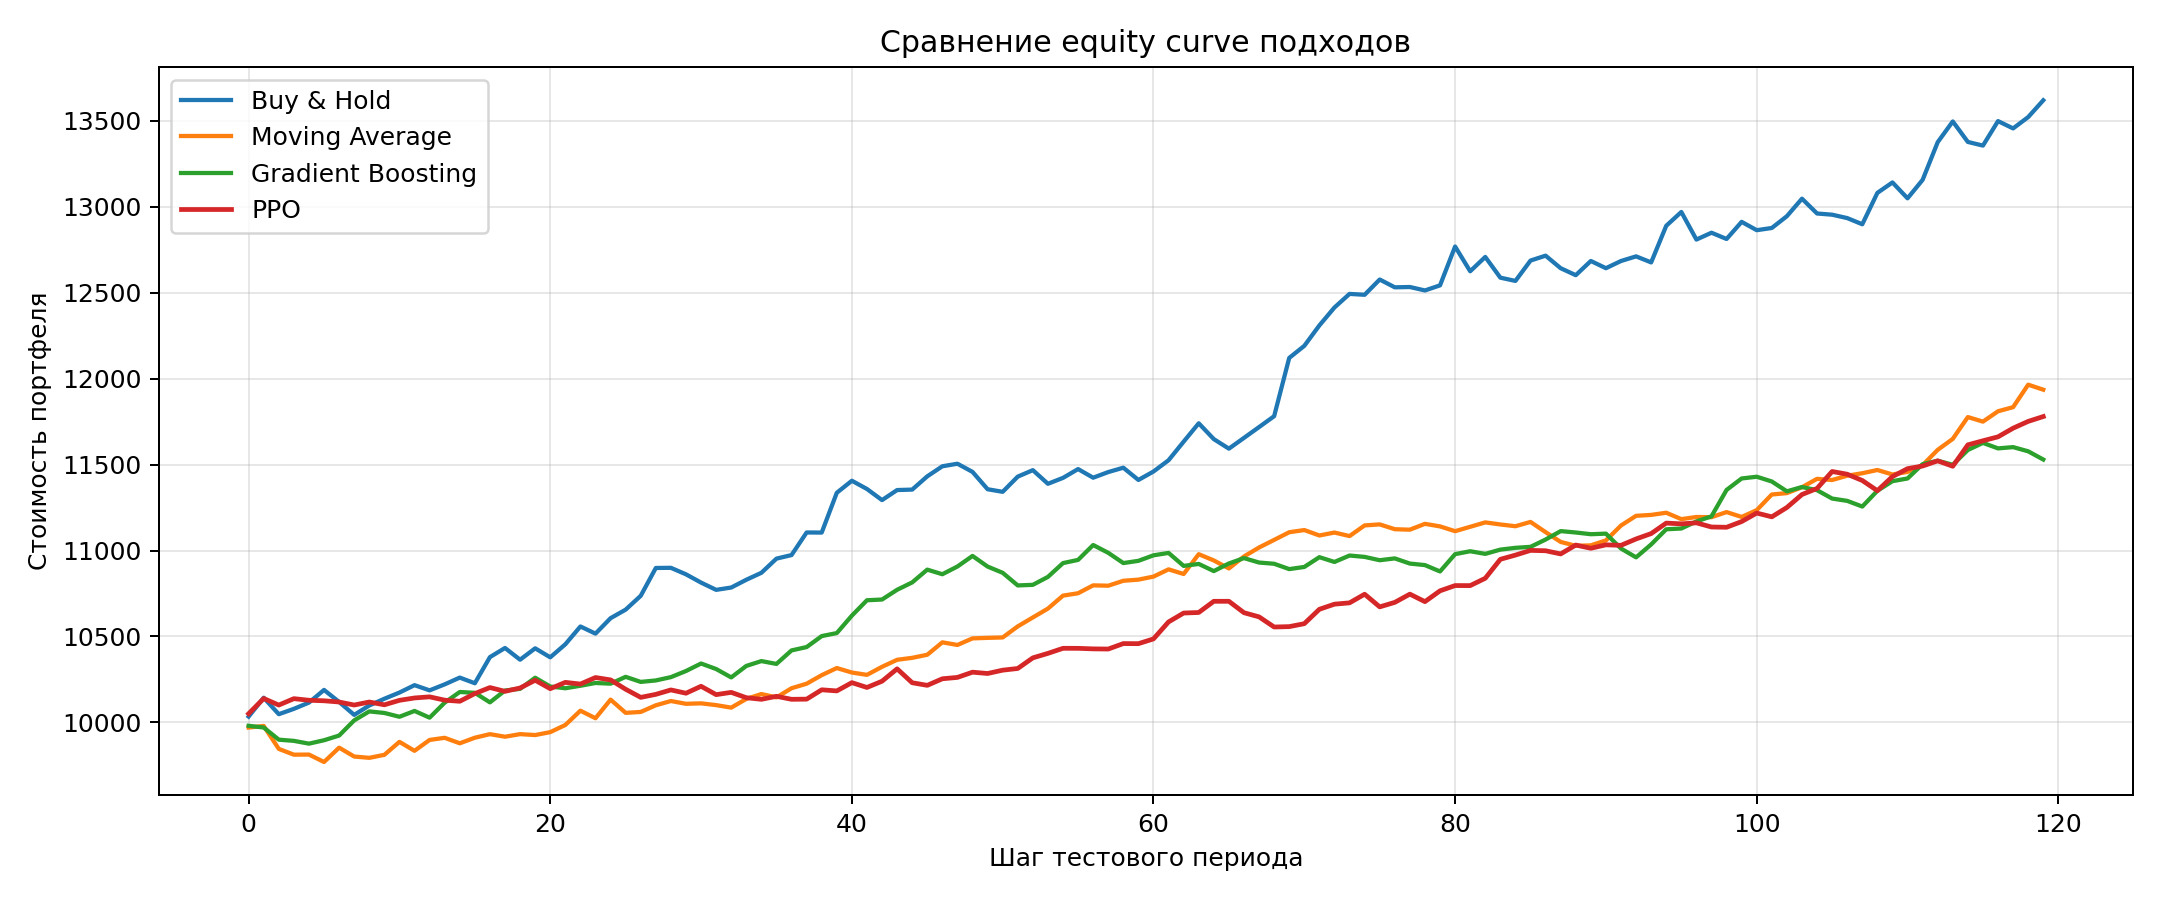
\includegraphics[width=0.92\textwidth]{equity_curves_comparison.png}
\caption{Сравнение equity curve различных подходов}
\label{fig:equity_curves_comparison}
\end{figure}

Рисунок~\ref{fig:equity_curves_comparison} показывает, что кривые капитала заметно различаются по форме. Пассивная стратегия дает наиболее сильный рост на трендовом участке, но сопровождается глубокими откатами. PPO и Gradient Boosting формируют более плавную траекторию капитала, что особенно важно для практической интерпретации результатов.

\subsection{Анализ риска и максимальной просадки}

Если перейти от абсолютной доходности к риску, картина становится менее однозначной. Buy \& Hold сопровождается самой глубокой просадкой, что логично для стратегии, постоянно находящейся в рынке. Moving Average Crossover снижает просадку за счет выхода из позиции в неблагоприятные фазы, но не обеспечивает столь же высокой доходности. Среди ML-подходов наименьшая просадка наблюдается у Gradient Boosting, а среди RL-подходов — у PPO.

\begin{figure}[H]
\centering
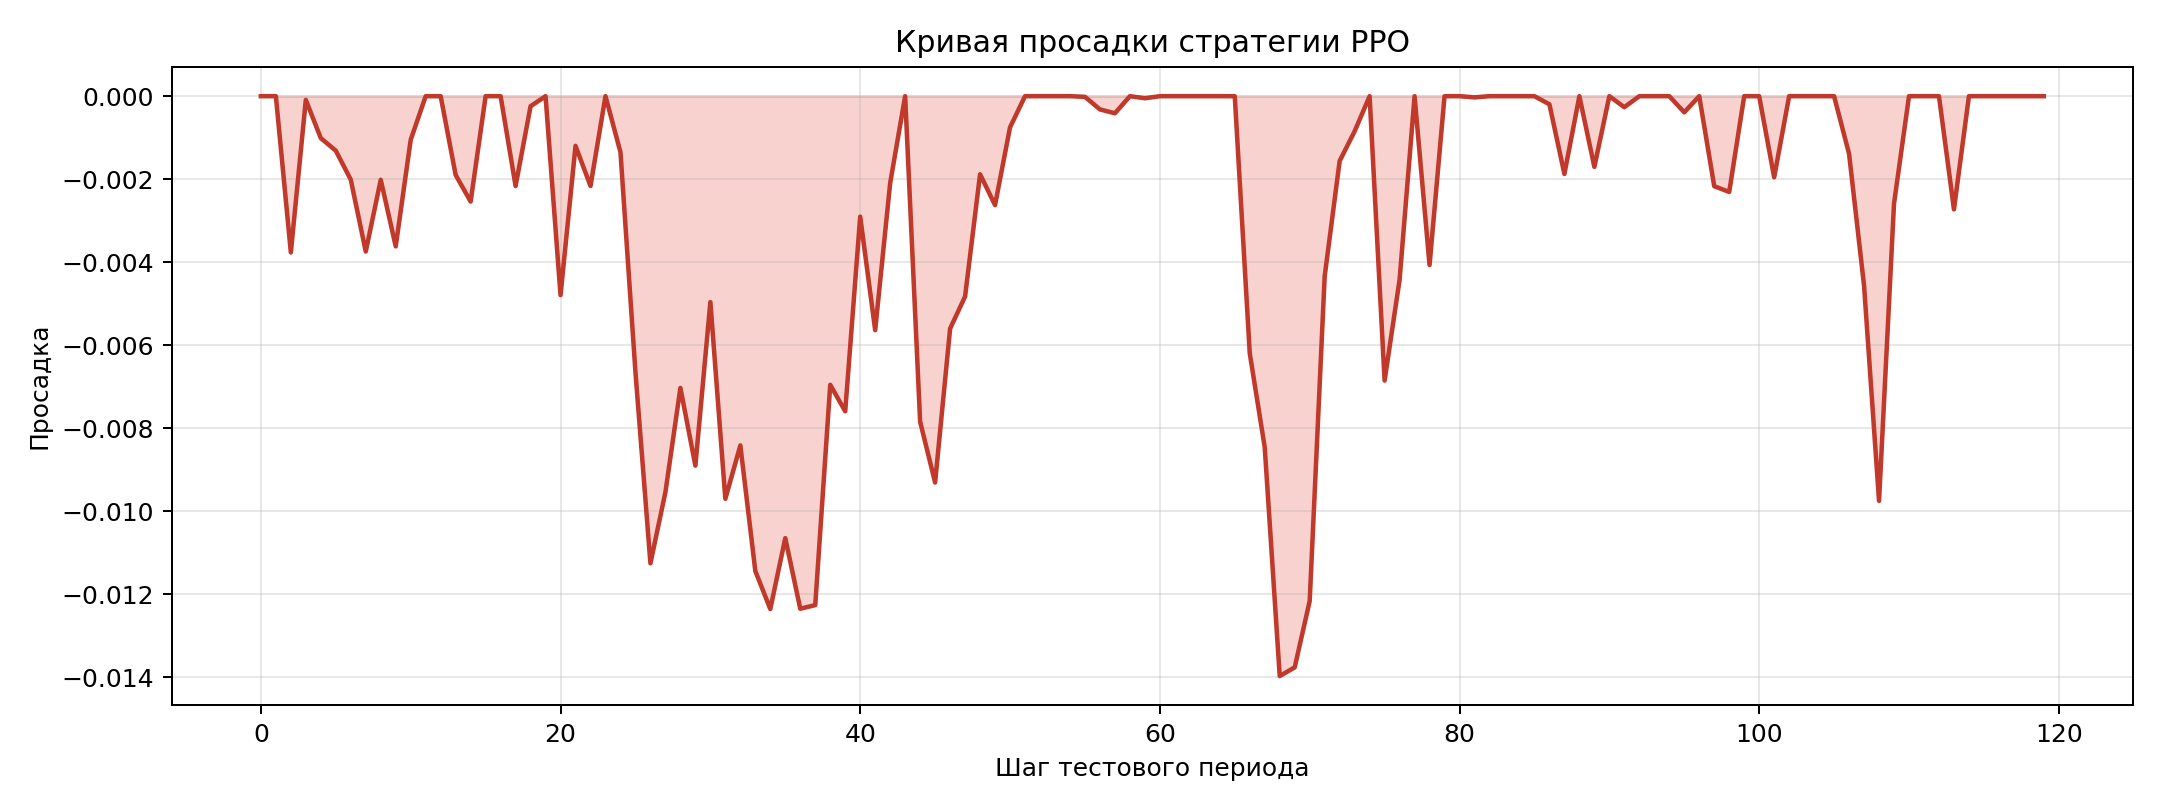
\includegraphics[width=0.92\textwidth]{drawdown_example.png}
\caption{Пример кривой просадки портфеля}
\label{fig:drawdown_example}
\end{figure}

На рисунке~\ref{fig:drawdown_example} видно, что глубина и продолжительность просадок являются не менее важными характеристиками стратегии, чем сама доходность. Для задач реального управления капиталом или даже учебной оценки устойчивости поведения алгоритма максимальная просадка часто имеет более прямой смысл, чем отдельные ML-метрики. Именно поэтому работа ориентируется на совмещенный анализ доходности и риска.

\subsection{Анализ устойчивости стратегий}

Под устойчивостью в работе понимается способность стратегии сохранять приемлемые характеристики не только в рамках единственного восходящего участка, но и при чередовании трендовых и боковых фаз рынка. В этом отношении простые baseline-стратегии и сложные RL-подходы демонстрируют различное поведение. Buy \& Hold стабилен в логике принятия решений, но нестабилен по просадке. Moving Average более устойчив в боковых и коррекционных участках, но платит за это потерей части доходности на сильных импульсах.

Среди ML-моделей наибольшую устойчивость в экспериментальном моделировании продемонстрировал Gradient Boosting: его сигналы оказались реже и качественнее, чем у Logistic Regression, и менее шумными, чем у части запусков Random Forest. PPO также показал достаточно сбалансированное поведение, в то время как DQN оказался более чувствителен к рыночному режиму. Это подтверждает гипотезу о том, что RL-агенты могут быть полезны в задачах последовательного управления позицией, но их устойчивость нельзя считать автоматически гарантированной.

\subsection{Ограничения проведенного исследования}

Несмотря на полученные результаты, исследование имеет ряд ограничений. Во-первых, рассматривается торговля одним активом в каждый момент времени без построения полноценного многоактивного портфеля. Во-вторых, используется упрощенная модель исполнения сделок, не учитывающая проскальзывание, глубину рынка и частичное исполнение заявок. В-третьих, набор признаков ограничен относительно компактным набором технических индикаторов и не включает новостные или макроэкономические факторы.

Кроме того, в рамках практической части полностью реализованы baseline-стратегии, три классические ML-модели и два RL-агента. Методы ARIMA/SARIMA, CatBoost/XGBoost, LSTM/GRU и A2C включены в обзор аналогов и методологическое сравнение, но не вошли в основной программный контур. Это решение принято осознанно: целью работы является построение понятного, воспроизводимого и умеренно ресурсоемкого программного решения, а не максимальное расширение набора моделей любой ценой.

Наконец, полученные численные результаты относятся к экспериментальному моделированию в рамках конкретной постановки задачи, конкретных признаков и выбранных интервалов данных. При изменении рыночного режима, функции награды, параметров среды или состава признаков итоговая сравнительная картина может измениться. По этой причине результаты эксперимента не являются инвестиционной рекомендацией и должны рассматриваться исключительно как итог проверки разработанного программного решения в учебно-исследовательских условиях.

\subsection{Выводы по главе}

Экспериментальное исследование показало, что сравнение торговых подходов требует многокритериальной оценки. Высокая точность прогноза не гарантирует высокой доходности, а высокая доходность не гарантирует приемлемого уровня риска. В условиях экспериментального моделирования стратегия Buy \& Hold сохранила лидерство по абсолютной совокупной доходности, тогда как PPO и Gradient Boosting продемонстрировали более сильные риск-скорректированные характеристики.

Полученные результаты позволяют сделать взвешенный вывод: обучение с подкреплением действительно имеет потенциал в задачах алгоритмической торговли, поскольку позволяет оптимизировать последовательность действий, а не только прогнозировать движение цены. Однако его ценность раскрывается только в сопоставлении с более простыми подходами и при строгой постановке эксперимента. Именно это и подтверждает ключевую идею разработанного программного решения и проведенной на нем экспериментальной проверки.

\clearpage
\section*{ЗАКЛЮЧЕНИЕ}
\addcontentsline{toc}{section}{ЗАКЛЮЧЕНИЕ}

Выпускная квалификационная работа была посвящена разработке и экспериментальной проверке программного решения для прогнозирования и оптимизации торговых решений на основе биржевых котировок с использованием методов обучения с подкреплением. В ходе работы была решена не только задача включения RL-алгоритмов в финансовую постановку, но и более широкая инженерная задача: создание единого программного контура, позволяющего корректно сравнивать baseline-стратегии, статистические методы, модели машинного обучения и RL-агентов.

В теоретической части были изучены особенности биржевых котировок как нестационарных финансовых временных рядов, рассмотрены классические подходы к прогнозированию, включая ARIMA/SARIMA, методы машинного обучения, нейросетевые архитектуры LSTM/GRU, а также RL-алгоритмы DQN, PPO и A2C. Отдельно был проведен обзор существующих аналогов и фреймворков — FinRL, TensorTrade и gym-anytrading. Это позволило выполнить требование о сравнении аналогов и показать, что предлагаемый подход не существует в вакууме, а занимает определенное место среди существующих исследовательских и прикладных решений.

В результате анализа была четко сформулирована проблема, которую решает работа. Обычное прогнозирование цены или направления движения недостаточно для практической оценки качества алгоритма, потому что высокая точность классификации не равна прибыльности торговой стратегии. Реальная ценность модели определяется тем, как ее сигналы влияют на динамику капитала, частоту сделок, глубину просадки и устойчивость на разных рыночных режимах. Поэтому центральным результатом работы стало построение программного стенда, в котором baseline-стратегии, ML-модели и RL-агенты сравниваются на одних и тех же данных по одинаковому набору финансовых и классификационных метрик.

В практической части реализован программный проект на Python с модульной структурой, включающей модуль загрузки данных через \texttt{yfinance}, модуль формирования OHLCV-датасета и признаков, модуль baseline-стратегий, модуль ML-моделей, торговую RL-среду на базе Gymnasium, модуль обучения агентов DQN и PPO через stable-baselines3, модуль backtesting, модуль расчета финансовых метрик и модуль визуализации результатов. Тем самым в работе не только описан теоретический подход, но и создано реальное программное решение, поддерживающее воспроизводимый запуск вычислительного эксперимента.

По итогам экспериментальной проверки разработанного ПО было показано, что:
\begin{enumerate}[leftmargin=1.25cm,label=\arabic*)]
\item стратегия Buy \& Hold сохраняет сильные позиции как простой и конкурентоспособный baseline, особенно на выраженном восходящем рынке;
\item стратегия на основе скользящих средних позволяет уменьшить просадку, но уступает пассивному удержанию по суммарной доходности на трендовом интервале;
\item среди реализованных ML-моделей наилучший баланс между качеством классификации и торговым результатом показал Gradient Boosting;
\item RL-подходы действительно способны использовать последовательную постановку задачи и оптимизировать торговые решения напрямую через функцию вознаграждения;
\item PPO оказался наиболее устойчивым из реализованных RL-агентов по совокупности риск-скорректированных метрик, тогда как DQN проявил большую чувствительность к параметрам среды и reward function.
\end{enumerate}

При этом результаты работы не дают основания утверждать, что RL всегда превосходит классические методы. Напротив, исследование показало, что качество RL-агента существенно зависит от выбора признаков, конфигурации среды, функции вознаграждения и характера рыночного режима. В ряде сценариев простые и интерпретируемые baseline-стратегии могут быть устойчивее и проще в сопровождении, а отдельные ML-модели способны демонстрировать конкурентоспособный результат при значительно меньшей вычислительной сложности.

Таким образом, основная ценность выполненной работы заключается не в декларации безусловного превосходства обучения с подкреплением, а в создании единого сравнительного программного стенда, позволяющего сопоставлять различные классы методов в корректной и воспроизводимой постановке. Разработанное решение может использоваться как основа для дальнейшего развития исследования и для расширения набора поддерживаемых торговых сценариев.

К числу перспективных направлений относятся: расширение набора признаков за счет макроэкономических и новостных данных, включение CatBoost/XGBoost, LSTM/GRU и A2C в основной экспериментальный контур, переход к многоактивному портфелю, использование walk-forward-валидации, моделирование проскальзывания и более сложных торговых ограничений, а также развитие reward function с учетом риска, просадки и стабильности стратегии.

Следовательно, цель работы достигнута: разработано, программно реализовано и экспериментально проверено решение для прогнозирования и оптимизации торговых решений на основе биржевых котировок, включающее модули загрузки данных, формирования признаков, реализации baseline- и ML-подходов, RL-среды, обучения агентов, backtesting, расчета метрик и визуализации результатов. Поставленные задачи решены, выпускная квалификационная работа выполнена в полном объеме.

\clearpage
\section*{СПИСОК ИСПОЛЬЗОВАННЫХ ИСТОЧНИКОВ}
\addcontentsline{toc}{section}{СПИСОК ИСПОЛЬЗОВАННЫХ ИСТОЧНИКОВ}

\begin{enumerate}[leftmargin=1cm,label=\arabic*.]
\item Sutton R.\,S., Barto A.\,G. Reinforcement Learning: An Introduction. 2nd ed. Cambridge: MIT Press, 2018. 552 p.
\item Hyndman R.\,J., Athanasopoulos G. Forecasting: Principles and Practice. 3rd ed. Melbourne: OTexts, 2021. 442 p.
\item Tsay R.\,S. Analysis of Financial Time Series. 3rd ed. Hoboken: Wiley, 2010. 720 p.
\item Box G.\,E.\,P., Jenkins G.\,M., Reinsel G.\,C., Ljung G.\,M. Time Series Analysis: Forecasting and Control. 5th ed. Hoboken: Wiley, 2015. 712 p.
\item Murphy J.\,J. Technical Analysis of the Financial Markets. New York: New York Institute of Finance, 1999. 576 p.
\item Chan E.\,P. Algorithmic Trading: Winning Strategies and Their Rationale. Hoboken: Wiley, 2013. 224 p.
\item López de Prado M. Advances in Financial Machine Learning. Hoboken: Wiley, 2018. 400 p.
\item Mnih V., Kavukcuoglu K., Silver D. et al. Human-level Control through Deep Reinforcement Learning // Nature. 2015. Vol. 518. P. 529--533.
\item Schulman J., Wolski F., Dhariwal P., Radford A., Klimov O. Proximal Policy Optimization Algorithms // arXiv preprint arXiv:1707.06347. 2017.
\item Mnih V., Badia A.\,P., Mirza M. et al. Asynchronous Methods for Deep Reinforcement Learning // Proceedings of the 33rd International Conference on Machine Learning. 2016. P. 1928--1937.
\item Hochreiter S., Schmidhuber J. Long Short-Term Memory // Neural Computation. 1997. Vol. 9, No. 8. P. 1735--1780.
\item Cho K., Van Merriënboer B., Gulcehre C. et al. Learning Phrase Representations using RNN Encoder--Decoder for Statistical Machine Translation // arXiv preprint arXiv:1406.1078. 2014.
\item Breiman L. Random Forests // Machine Learning. 2001. Vol. 45. P. 5--32.
\item Friedman J.\,H. Greedy Function Approximation: A Gradient Boosting Machine // The Annals of Statistics. 2001. Vol. 29, No. 5. P. 1189--1232.
\item Pedregosa F., Varoquaux G., Gramfort A. et al. Scikit-learn: Machine Learning in Python // Journal of Machine Learning Research. 2011. Vol. 12. P. 2825--2830.
\item Harris C.\,R., Millman K.\,J., van der Walt S.\,J. et al. Array Programming with NumPy // Nature. 2020. Vol. 585. P. 357--362.
\item McKinney W. Data Structures for Statistical Computing in Python // Proceedings of the 9th Python in Science Conference. 2010. P. 56--61.
\item Paszke A., Gross S., Massa F. et al. PyTorch: An Imperative Style, High-Performance Deep Learning Library // Advances in Neural Information Processing Systems. 2019. Vol. 32. P. 8024--8035.
\item Raffin A., Hill A., Gleave A., Kanervisto A., Ernestus M., Dormann N. Stable-Baselines3: Reliable Reinforcement Learning Implementations // Journal of Machine Learning Research. 2021. Vol. 22. P. 1--8.
\item Towers M., Terry J.\,K., Kwiatkowski A. et al. Gymnasium // GitHub repository. URL: https://gymnasium.farama.org/ (дата обращения: 28.04.2026).
\item Yang H., Liu X.-Y., Zhong S., Walid A. FinRL: A Deep Reinforcement Learning Library for Automated Stock Trading in Quantitative Finance // NeurIPS 2020 Workshop on Financial Technology and FinRL. 2020.
\item The TensorTrade Authors. TensorTrade Documentation. URL: https://tensortrade-ng.io/ (дата обращения: 28.04.2026).
\item AminHP. gym-anytrading Documentation. URL: https://github.com/AminHP/gym-anytrading (дата обращения: 28.04.2026).
\item Yahoo Finance API via yfinance Documentation. URL: https://github.com/ranaroussi/yfinance (дата обращения: 28.04.2026).
\item Fama E.\,F. Efficient Capital Markets: A Review of Theory and Empirical Work // The Journal of Finance. 1970. Vol. 25, No. 2. P. 383--417.
\item Lo A.\,W., MacKinlay A.\,C. A Non-Random Walk Down Wall Street. Princeton: Princeton University Press, 1999. 288 p.
\item Bailey D., López de Prado M. The Sharpe Ratio Efficient Frontier // Journal of Risk. 2012. Vol. 15, No. 2. P. 3--44.
\item Magdon-Ismail M., Atiya A.\,F. Maximum Drawdown // Risk Magazine. 2004. Vol. 17, No. 10. P. 99--102.
\end{enumerate}

\clearpage
\section*{ПРИЛОЖЕНИЕ А}
\addcontentsline{toc}{section}{ПРИЛОЖЕНИЕ А}

\begin{flushright}
\textbf{Приложение А}
\end{flushright}

\begin{center}
\textbf{СТРУКТУРА ПРОГРАММНОГО ПРОЕКТА И ПРИМЕРЫ ЗАПУСКА}
\end{center}

В приложении приведена укрупненная структура программного проекта, разработанного в рамках настоящей выпускной квалификационной работы.

\begin{verbatim}
diploma_rl_trading/
├── data/
├── notebooks/
├── src/
│   ├── data/
│   ├── strategies/
│   ├── models/
│   ├── rl/
│   ├── metrics/
│   └── visualization/
├── reports/
├── requirements.txt
└── main.py
\end{verbatim}

Назначение ключевых элементов структуры:
\begin{enumerate}[leftmargin=1.25cm,label=\arabic*)]
\item каталог \texttt{data/} используется для хранения исходных и обработанных котировок;
\item каталог \texttt{notebooks/} предназначен для исследовательских записных книжек и промежуточного анализа;
\item каталог \texttt{src/} содержит основную логику системы, разбитую по функциональным модулям;
\item каталог \texttt{reports/} служит для сохранения метрик, таблиц, графиков и прочих результатов экспериментов;
\item файл \texttt{requirements.txt} фиксирует зависимости проекта;
\item файл \texttt{main.py} запускает полный сравнительный pipeline.
\end{enumerate}

Ниже приведены примеры команд, использованных в рамках экспериментального моделирования:

\begin{verbatim}
python3 main.py --ticker AAPL --start_date 2018-01-01 --end_date 2024-01-01 \
  --initial_cash 10000 --transaction_cost 0.001 --random_state 42

python3 src/rl/train_ppo.py --data_path data/processed/aapl_features.csv \
  --ticker AAPL --timesteps 20000 --initial_cash 10000 --transaction_cost 0.001

python3 src/rl/train_dqn.py --data_path data/processed/aapl_features.csv \
  --ticker AAPL --timesteps 15000 --initial_cash 10000 --transaction_cost 0.001
\end{verbatim}

Представленная структура проекта обеспечивает воспроизводимость вычислительного эксперимента и позволяет последовательно расширять стенд за счет новых признаков, алгоритмов и сценариев оценки.


\end{document}
